% !TeX root = ../main.tex
\documentclass[../main.tex]{subfiles}

\begin{document}
\chapter{Ecuaciones de onda electromagnéticas en el vacío}

\section{Desacople del sistema y ecuación de onda para el campo eléctrico}

\textbf{El siguiente objetivo es desacoplar parcialmente el sistema de Maxwell} para obtener una ecuación de segundo orden para el campo eléctrico. Partimos de la ley de Ampère-Maxwell,
\begin{equation}
    \vec \nabla \times \B = \mu_0\J+\mu_0\varepsilon_0\frac{\partial\E}{\partial t}.
    \label{eq:ampere-onda-E}
\end{equation}
Derivando \eqref{eq:ampere-onda-E} respecto del tiempo, se obtiene
\begin{equation*}
    \frac{\partial}{\partial t}\left(\vec \nabla \times \B\right)=\frac{\partial}{\partial t}\left(\mu_0\J+\mu_0\varepsilon_0\frac{\partial\E}{\partial t}\right).
\end{equation*}
Usando la conmutación de derivadas \eqref{eq:conmutacion-rotor-tiempo}, la ecuación anterior se reescribe como
\begin{equation*}
   \vec \nabla \times \frac{\partial\B}{\partial t}=\mu_0\frac{\partial\J}{\partial t}+\mu_0\varepsilon_0\frac{\partial^2\E}{\partial t^2}.
\end{equation*}
Ahora sustituimos la derivada temporal del campo magnético usando la ley de Faraday \eqref{eq:maxwell-faraday}. Así, resulta
\begin{equation*}
   \vec \nabla \times \left(-\vec\nabla\times \E\right)=\mu_0\frac{\partial\J}{\partial t}+\mu_0\varepsilon_0\frac{\partial^2\E}{\partial t^2}.
\end{equation*}
Recordando la identidad vectorial
\begin{equation}
    \vec \nabla \times (\vec \nabla \times \vec A)=\vec\nabla(\vec\nabla\cdot \vec A)-\nabla^2\vec A,
    \label{eq:identidad-rotrot}
\end{equation}
esta ecuación se convierte en
\begin{equation*}
  \nabla^2\vec E- \vec\nabla(\vec\nabla\cdot \E)= \mu_0\frac{\partial\J}{\partial t}+\mu_0\varepsilon_0\frac{\partial^2\E}{\partial t^2}.
\end{equation*}
Usando ahora la ley de Gauss eléctrica \eqref{eq:maxwell-gauss-E}, la ecuación anterior toma la forma
\begin{equation*}
  \nabla^2\vec E- \vec\nabla\left(\frac{\rho}{\varepsilon_0}\right)= \mu_0\frac{\partial\J}{\partial t}+\mu_0\varepsilon_0\frac{\partial^2\E}{\partial t^2}.
\end{equation*}
Reordenando los términos de la ecuación anterior para dejar en el miembro izquierdo sólo el campo eléctrico, se obtiene la \textbf{ecuación de onda inhomogénea para $\E$},
\begin{equation}
  \nabla^2\vec E- \mu_0\varepsilon_0\frac{\partial^2\E}{\partial t^2}=\frac{1}{\varepsilon_0}\vec\nabla \rho+\mu_0\frac{\partial\J}{\partial t}.
  \label{eq:ecuacion-onda-E}
\end{equation}

Aquí conviene comparar \eqref{eq:ecuacion-onda-E} con la forma general de una ecuación de onda escalar,
\begin{equation}
    \nabla^2\psi-\frac{1}{v^2}\frac{\partial^2\psi}{\partial t^2}=\text{fuentes}.
    \label{eq:ecuacion-onda-escalar-general}
\end{equation}
Comparando \eqref{eq:ecuacion-onda-E} con \eqref{eq:ecuacion-onda-escalar-general}, se identifica
\begin{equation*}
    \frac{1}{v^2}=\mu_0\varepsilon_0,
\end{equation*}
y, por tanto,
\begin{equation*}
    c=\frac{1}{\sqrt{\varepsilon_0 \mu_0}}.
\end{equation*}
\textbf{El desacople matemático de Maxwell conduce así, de manera completamente natural, a una velocidad de propagación que coincide con la velocidad de la luz en el vacío.}

\section{Ecuación de onda para el campo magnético}

De manera análoga, ahora obtenemos la ecuación de onda del campo magnético. Partimos de la ley de Faraday \eqref{eq:maxwell-faraday} y derivamos respecto del tiempo:
\begin{equation*}
    \frac{\partial }{\partial t}\left(\vec \nabla \times \E\right)=\frac{\partial }{\partial t}\left(-\frac{\partial \B}{\partial t}\right).
\end{equation*}
Usando de nuevo la conmutación de derivadas, esta ecuación se escribe como
\begin{equation*}
    \vec \nabla \times \frac{\partial \E}{\partial t}= -\frac{\partial^2 \B}{\partial t^2}.
\end{equation*}
Multiplicamos ahora esta ecuación por $\mu_0\varepsilon_0$ y reagrupamos el miembro izquierdo:
\begin{equation*}
    \vec \nabla \times \left(\mu_0\varepsilon_0\frac{\partial \E}{\partial t}\right)= -\mu_0\varepsilon_0\frac{\partial^2 \B}{\partial t^2}.
\end{equation*}
Por la ley de Ampère-Maxwell \eqref{eq:maxwell-ampere}, se tiene
\begin{equation*}
    \mu_0\varepsilon_0\frac{\partial \E}{\partial t}=\vec\nabla\times\B-\mu_0\J.
\end{equation*}
Sustituyendo \eqref{eq:maxwell-ampere} en la ecuación anterior, resulta
\begin{equation*}
    \vec \nabla \times \left(\vec\nabla\times\B-\mu_0\J\right)= -\mu_0\varepsilon_0\frac{\partial^2 \B}{\partial t^2}.
\end{equation*}
Distribuyendo el rotor en esta expresión, se obtiene
\begin{equation*}
    \vec \nabla \times \left(\vec\nabla\times\B\right)-\mu_0\vec \nabla \times \J= -\mu_0\varepsilon_0\frac{\partial^2 \B}{\partial t^2}.
\end{equation*}
Usando la identidad \eqref{eq:identidad-rotrot}, con $\vec A=\B$, se sigue que
\begin{equation*}
    \vec\nabla(\vec\nabla\cdot\vec B)-\nabla^2\vec B-\mu_0\vec \nabla \times \J= -\mu_0\varepsilon_0\frac{\partial^2 \B}{\partial t^2}.
\end{equation*}
Ahora usamos la ley de Gauss magnética \eqref{eq:maxwell-gauss-B}, es decir, $\vec\nabla\cdot\B=0$. Entonces esta ecuación se reduce a
\begin{equation*}
    -\nabla^2\vec B-\mu_0\vec \nabla \times \J= -\mu_0\varepsilon_0\frac{\partial^2 \B}{\partial t^2}.
\end{equation*}
Reordenando los términos de la ecuación anterior, obtenemos la \textbf{ecuación de onda inhomogénea para $\B$},
\begin{equation*}
    \nabla^2\vec B-\mu_0\varepsilon_0\frac{\partial^2 \B}{\partial t^2}= -\mu_0\vec \nabla \times \J.
\end{equation*}
Esta forma es equivalente a escribir todos los términos con signo opuesto; la física es la misma.

\section{Por qué las ecuaciones de onda no bastan por sí solas}

Las ecuaciones de onda obtenidas para $\E$ y $\B$ constituyen \textbf{condiciones necesarias, pero no suficientes}, para satisfacer el sistema completo de Maxwell. En efecto, al desacoplar el sistema y pasar a ecuaciones de segundo orden se pierde parte de la información contenida en las ecuaciones originales de primer orden, en particular las restricciones de divergencia y las relaciones mutuas entre ambos campos. Una pareja de campos puede satisfacer las ecuaciones de onda y, sin embargo, no satisfacer simultáneamente
\begin{equation*}
    \vec\nabla\cdot\E=\frac{\rho}{\varepsilon_0},
    \qquad
    \vec\nabla\cdot\B=0,
    \qquad
    \vec\nabla\times\E=-\frac{\partial\B}{\partial t},
    \qquad
    \vec\nabla\times\B=\mu_0\J+\mu_0\varepsilon_0\frac{\partial\E}{\partial t}.
\end{equation*}
Por consiguiente, las ecuaciones de onda deben entenderse como consecuencias del sistema de Maxwell, pero no como un sustituto de éste.

\begin{cuidado}
Siempre que se obtengan soluciones a partir de las ecuaciones de onda, es necesario verificar al final las ecuaciones de divergencia y las relaciones de rotor que constituyen el contenido completo de Maxwell.
\end{cuidado}

En regiones libres de fuentes, es decir, cuando $\rho=0$ y $\vec J=0$, las ecuaciones de onda para los campos eléctrico y magnético quedan dadas por ecuaciones diferenciales de segundo orden homogéneas,
\begin{equation*}
    \Box\E=\vec 0,
    \qquad
    \Box\B=\vec 0,
\end{equation*}
donde se define el operador de onda
\begin{equation*}
    \Box=\frac{1}{c^2}\frac{\partial^2}{\partial t^2}-\nabla^2.
\end{equation*}



% La discusión detallada sobre la conexión con óptica ondulatoria se trasladó al apéndice.


\textbf{Para una discusión más detallada sobre la relación entre esta estructura ondulatoria y el formalismo escalar usual de la óptica ondulatoria, véase el Apéndice~\ref{ap:optica-ondulatoria}. Allí se resume la conexión con la ecuación de onda escalar, el principio de superposición, la representación compleja y la ecuación de Helmholtz.}

\section{Ondas planas monocromáticas con polarización lineal}

Buscaremos ahora soluciones particulares de estas ecuaciones en ausencia de fuentes. Consideremos, en primer lugar, una \textbf{onda electromagnética plana monocromática con polarización lineal}:
\begin{equation*}
    \E(\vec x,t)= \vec E_0\cos\left(\vec k\cdot \vec x -\omega t+\varphi_0\right)
\end{equation*}
\begin{equation*}
    \B(\vec x,t)= \vec B_0\cos\left(\vec k\cdot \vec x -\omega t+\varphi_0\right).
\end{equation*}
Aquí $\vec E_0$ y $\vec B_0$ son vectores constantes que representan las amplitudes de las ondas, $\vec k$ es el vector de onda, cuya dirección fija la dirección de propagación, $\omega$ es la frecuencia angular constante ---de ahí que la onda sea monocromática--- y $\varphi_0$ es una fase inicial.


%%%%%%%%%%%%%%%%%%%%%%%%%%%%%%%%%%%%%%%%%%%%%%%%%%%%%%%%%%%%%%%%%%%%%%%%%%%%%%%%%%%%%%%%%%%%%%%%%%%%%%%%%%%%%%%%%

Sea
\begin{equation*}
    \Phi(\vec x,t)=\vec k\cdot \vec x-\omega t+\varphi_0
\end{equation*}
la fase de la onda. Un \textbf{frente de onda} es el lugar geométrico de los puntos del espacio para los cuales la fase permanece constante. En otras palabras, los frentes de onda son las superficies
\begin{equation*}
    \Phi(\vec x,t)=\text{cte}.
\end{equation*}

En el caso particular de una onda plana monocromática, a tiempo fijo $t=t_0$, la condición anterior se reduce a
\begin{equation*}
    \vec k\cdot \vec x=\text{cte},
\end{equation*}
de modo que los frentes de onda son planos perpendiculares al vector de onda $\vec k$. Por tanto, $\vec k$ fija la dirección de propagación de la onda.

Si $\nu$ es la frecuencia ordinaria, $\omega$ la frecuencia angular y $T$ el período, entonces
\begin{equation*}
    \nu=\frac{1}{T},
    \qquad
    \omega=2\pi \nu=\frac{2\pi}{T}.
\end{equation*}
En unidades del SI,
\begin{equation*}
    [\nu]=\mathrm{Hz},
    \qquad
    [\omega]=\mathrm{rad\,s^{-1}},
    \qquad
    [T]=\mathrm{s}.
\end{equation*}

\textbf{La longitud de onda se obtiene comparando dos frentes consecutivos}. Si nos desplazamos una distancia $\lambda$ en la dirección $\hat k=\vec k/k$, la fase debe cambiar en $2\pi$:
\begin{equation*}
    \Phi(\vec x+\lambda \hat k,t)-\Phi(\vec x,t)=2\pi.
\end{equation*}
Como $\vec k\cdot \hat k=k$, se sigue que
\begin{equation*}
    k\lambda=2\pi,
\end{equation*}
y, por tanto,
\begin{equation*}
    \lambda=\frac{2\pi}{k}.
\end{equation*}



\begin{figure}[ht]
    \centering
    \begingroup
    \shorthandoff{<>}
    \begin{tikzpicture}[scale=1.0,>=Latex,line join=round,line cap=round]
        \def\ang{-16}
        \def\h{2.15}
        \def\w{1.15}
        \def\sep{3.75}
        \coordinate (S) at ({\ang}:\sep);
        \begin{scope}[shift={(-0.25,-0.10)}]
            \coordinate (A) at ({\ang+90}:\h);
            \coordinate (B) at ({\ang-90}:\h);
            \coordinate (C) at ($ (B)+(10:\w) $);
            \coordinate (D) at ($ (A)+(10:\w) $);
            \fill[UdeCAzul!8] (A)--(B)--(C)--(D)--cycle;
            \draw[very thick,UdeCAzul!80!black] (A)--(B)--(C)--(D)--cycle;
            \node[font=\small,UdeCAzul!80!black,fill=white,inner sep=1pt] at ($ (A)!0.5!(D)+(0,0.35) $) {$t$};
        \end{scope}
        \begin{scope}[shift={($ (S)+(-0.25,-0.10) $)}]
            \coordinate (A) at ({\ang+90}:\h);
            \coordinate (B) at ({\ang-90}:\h);
            \coordinate (C) at ($ (B)+(10:\w) $);
            \coordinate (D) at ($ (A)+(10:\w) $);
            \fill[UdeCDorado!10] (A)--(B)--(C)--(D)--cycle;
            \draw[very thick,UdeCDorado!85!black] (A)--(B)--(C)--(D)--cycle;
            \node[font=\small,UdeCDorado!85!black,fill=white,inner sep=1pt] at ($ (A)!0.5!(D)+(0,0.35) $) {$t+\Delta t$};
        \end{scope}
        \coordinate (C1) at (0.35,0.15);
        \coordinate (C2) at ($ (C1)+(S) $);
        \draw[vecazul] (C1) -- (C2) node[midway,above=6pt,sloped,fill=white,inner sep=1pt] {$\vec k$};
        \coordinate (Q1) at ($ (C1)+({\ang-90}:1.18) $);
        \coordinate (Q2) at ($ (C2)+({\ang-90}:1.18) $);
        \draw[dashed,gray!55] (C1)--(Q1);
        \draw[dashed,gray!55] (C2)--(Q2);
        \draw[<->,gray!75!black] (Q1)--(Q2) node[midway,below=5pt,sloped,fill=white,inner sep=1pt] {$\Delta x$};
        \node[cajadiagrama, text width=6.2cm] at (2.35,3.0)
        {$\Phi(\vec x,t)=\vec k\cdot\vec x-\omega t+\varphi_0$\\
        un frente de onda cumple $\Phi=\mathrm{cte}$};
        \node[font=\small,align=center,gray!70!black,fill=white,inner sep=2pt] at (2.25,-3.75)
        {seguir el mismo valor de fase implica\\$k\Delta x=\omega\Delta t$};
    \end{tikzpicture}
    \endgroup
    \caption{Desplazamiento de una superficie de fase constante de una onda plana monocromática. La figura separa el objeto geométrico ---el frente de fase--- de la dirección de propagación fijada por $\vec k$.}
    \label{fig:avance-frente-fase}
\end{figure}




Si ahora seguimos un punto de fase constante en la dirección de propagación, entonces
\begin{equation*}
    \Phi(\vec x+\Delta x\,\hat k,t+\Delta t)=\Phi(\vec x,t).
\end{equation*}
De aquí se obtiene
\begin{equation*}
    k\,\Delta x=\omega\,\Delta t,
\end{equation*}
y, por tanto, la velocidad de fase resulta ser
\begin{equation*}
    v_{\mathrm f}=\frac{\Delta x}{\Delta t}=\frac{\omega}{k}=\nu\lambda.
\end{equation*}

En una onda electromagnética, la \textbf{polarización} queda determinada por la dirección en que oscila el campo eléctrico. En particular, si el campo eléctrico oscila siempre paralelo a un mismo vector constante $\vec E_0$, entonces la onda está \textbf{linealmente polarizada}. Lo esencial aquí no es que $\vec k$ sea constante, sino que la dirección de $\vec E_0$ permanezca fija. El ojo humano, por sí solo, no percibe directamente la polarización de la luz; detecta principalmente su intensidad.


\begin{figure}[ht]
    \centering
    \begingroup
    \shorthandoff{<>}
    \begin{tikzpicture}[scale=0.96,>=Latex,line join=round,line cap=round]
        \coordinate (O) at (0,0);
        \draw[eje] (O) -- (0,2.9) node[above] {$\hat e_x$};
        \draw[eje] (O) -- (-1.70,-1.05) node[left] {$\hat e_y$};
        \draw[eje] (O) -- (9.55,0) node[right] {$\hat e_z$};
        \foreach \z/\op in {1.55/0.95,3.30/0.82,5.05/0.68,6.80/0.54,8.55/0.40}
        {
            \begin{scope}[shift={(\z,0)}]
                \fill[UdeCAzul!8,opacity=\op] (-0.50,-0.85)--(-0.50,0.95)--(0.58,1.28)--(0.58,-0.52)--cycle;
                \draw[UdeCAzul!75!black,thick] (-0.50,-0.85)--(-0.50,0.95)--(0.58,1.28)--(0.58,-0.52)--cycle;
            \end{scope}
        }
        \draw[vecazul] (0.75,0.47) -- (9.20,0.47)
            node[midway,above=6pt,fill=white,inner sep=1pt] {$\vec k=k\hat e_z$};
        \foreach \z in {2.0,4.0,6.0,8.0}
        {
            \draw[vecverde] (\z,0) -- (\z,1.00);
            \node[font=\small,green!45!black,fill=white,inner sep=1pt] at (\z,1.25) {$\E$};
            \draw[vecdorado] (\z,0) -- ($ (\z,0)+(-0.72,-0.48) $);
            \node[font=\small,UdeCDorado!85!black,fill=white,inner sep=1pt] at ($ (\z,0)+(-0.88,-0.68) $) {$\B$};
        }
        \draw[<->,gray!70!black] (1.55,-1.35) -- (3.30,-1.35) node[midway,below=3pt,fill=white,inner sep=1pt] {$\lambda$};
        \node[cajadiagrama, text width=5.15cm] at (5.25,3.05)
        {$\E\perp\B$, $\E\perp\vec k$, $\B\perp\vec k$\\[2pt]
        $\displaystyle \B=\frac{1}{c}\hat k\times\E$};
    \end{tikzpicture}
    \endgroup
    \caption{Onda plana monocromática propagándose en la dirección $\vec k\parallel\hat e_z$. Los frentes de onda son planos perpendiculares a $\vec k$ y los campos son transversales a la propagación.}
    \label{fig:onda-plana-campos-transversales}
\end{figure}




\begin{figure}[ht]
    \centering
    \begingroup
    \shorthandoff{<>}
    \begin{tikzpicture}[x=0.92cm,y=1cm,>=Latex,line join=round,line cap=round]
        \def\lam{6.0}
        \def\A{1.30}
        \def\xmax{11.2}
        \draw[eje] (-0.35,0) -- (\xmax+0.75,0) node[right] {$z$};
        \draw[eje] (0,-2.05) -- (0,3.05) node[above] {$E_x$};
        \draw[densely dashed,gray!55] (0,\A) -- (\xmax,\A);
        \draw[densely dashed,gray!55] (0,-\A) -- (\xmax,-\A);
        \node[left] at (0,\A) {$E_0$};
        \node[left] at (0,-\A) {$-E_0$};
        \draw[UdeCAzul!80!black,very thick,smooth,samples=240,domain=0:\xmax]
            plot (\x,{\A*cos(360*\x/\lam)});
        \foreach \n in {0,...,16}
        {
            \pgfmathsetmacro{\xx}{0.35 + 0.64*\n}
            \pgfmathsetmacro{\Ey}{\A*cos(360*\xx/\lam)}
            \draw[vecazul] (\xx,0) -- (\xx,\Ey);
        }
        \draw[decorate, decoration={brace, mirror, amplitude=5pt}]
            (0,-1.68) -- (\lam,-1.68) node[midway,below=7pt] {$\lambda$};
        \node[cajadiagrama, text width=4.85cm] at (8.25,2.72)
        {polarización lineal:\\la dirección de $\E$ es fija,\\sólo cambia su magnitud y signo};
        \node[font=\small,fill=white,inner sep=2pt] at (3.0,1.85) {$t=t_0$};
    \end{tikzpicture}
    \endgroup
    \caption{Instantánea espacial de una onda plana linealmente polarizada. Las flechas muestran que el campo eléctrico oscila sobre una recta fija del plano transversal.}
    \label{fig:polarizacion-lineal-instantanea}
\end{figure}



La onda plana monocromática linealmente polarizada es una idealización útil, pero extrema: ningún sistema físico real produce una onda de esta forma en todo el espacio y durante todo el tiempo. Sin embargo, este modelo describe muy bien, de manera aproximada, la radiación en regiones pequeñas comparadas con la distancia a la fuente, o bien haces suficientemente colimados en zonas donde la curvatura de los frentes de onda puede despreciarse. Además, este tipo de soluciones desempeña un papel central en el análisis de Fourier y en la construcción de soluciones más generales de las ecuaciones de Maxwell.

También es muy conveniente introducir la representación compleja del campo eléctrico:
\begin{align*}
    \E(\vec x,t)
    &= \vec E_0 \cos\left(\vec k\cdot\vec x-\omega t+\varphi_0\right) \\
    &= \operatorname{Re}\left[\vec E_{0,c}\,\ee^{\ii\left(\vec k\cdot\vec x-\omega t\right)}\right],
\end{align*}
donde
\begin{equation*}
    \vec E_{0,c}=\vec E_0\,\ee^{\ii\varphi_0}
\end{equation*}
es la amplitud compleja del campo eléctrico. De manera análoga,
\begin{align*}
    \B(\vec x,t)
    &= \vec B_0 \cos\left(\vec k\cdot\vec x-\omega t+\varphi_0\right) \\
    &= \operatorname{Re}\left[\vec B_{0,c}\,\ee^{\ii\left(\vec k\cdot\vec x-\omega t\right)}\right],
\end{align*}
con
\begin{equation*}
    \vec B_{0,c}=\vec B_0\,\ee^{\ii\varphi_0}.
\end{equation*}

En el vacío, las ecuaciones de Maxwell implican que ambos campos satisfacen la ecuación de onda
\begin{equation*}
    \Box \E
    =\left(\frac{1}{c^2}\frac{\partial^2}{\partial t^2}-\nabla^2\right)\E
    =\vec 0,
    \qquad
    c=\frac{1}{\sqrt{\epsz\muz}}.
\end{equation*}
Sustituyendo el ansatz de onda plana monocromática se obtiene
\begin{align*}
    \Box \E
    &=\left(\frac{1}{c^2}\frac{\partial^2}{\partial t^2}-\nabla^2\right)
      \left[\vec E_0\cos\left(\vec k\cdot\vec x-\omega t+\varphi_0\right)\right] \\
    &=\frac{1}{c^2}\left[-\omega^2\,\vec E_0\cos\left(\vec k\cdot\vec x-\omega t+\varphi_0\right)\right]
      -\left[-k^2\,\vec E_0\cos\left(\vec k\cdot\vec x-\omega t+\varphi_0\right)\right] \\
    &=\left(k^2-\frac{\omega^2}{c^2}\right)\E(\vec x,t).
\end{align*}
Para que esta expresión se anule en todo punto, debe cumplirse
\begin{equation*}
    k^2-\frac{\omega^2}{c^2}=0,
\end{equation*}
es decir,
\begin{equation*}
    \omega^2=c^2k^2.
\end{equation*}
Tomando $\omega>0$ y $k>0$, se obtiene la relación de dispersión
\begin{equation*}
    \omega=ck.
\end{equation*}
Por consiguiente, en el vacío
\begin{equation*}
    v_{\mathrm f}=\frac{\omega}{k}=c.
\end{equation*}
Además, como la relación de dispersión es lineal, la velocidad de grupo también coincide con $c$:
\begin{equation*}
    v_{\mathrm g}=\frac{\partial \omega}{\partial k}=c.
\end{equation*}

Veamos ahora qué restricciones adicionales imponen las ecuaciones de Maxwell sobre las amplitudes $\vec E_0$ y $\vec B_0$. En una región libre de fuentes se tiene
\begin{equation*}
    \diver \E=0,
    \qquad
    \diver \B=0,
    \qquad
    \rot \E+\frac{\partial \B}{\partial t}=\vec 0,
    \qquad
    \rot \B-\frac{1}{c^2}\frac{\partial \E}{\partial t}=\vec 0.
\end{equation*}

A partir de la ley de Gauss para el campo eléctrico,
\begin{align*}
    0
    =\diver \E
    &=\diver\left[\vec E_0\cos\left(\vec k\cdot\vec x-\omega t+\varphi_0\right)\right] \\
    &=\vec E_0\cdot\nabla\cos\left(\vec k\cdot\vec x-\omega t+\varphi_0\right) \\
    &=-(\vec k\cdot\vec E_0)\sin\left(\vec k\cdot\vec x-\omega t+\varphi_0\right).
\end{align*}
Como esta igualdad debe cumplirse para todo $\vec x$ y todo $t$, necesariamente
\begin{equation*}
    \vec k\cdot \vec E_0=0.
\end{equation*}
De manera completamente análoga, a partir de $\diver \B=0$ se obtiene
\begin{equation*}
    \vec k\cdot \vec B_0=0.
\end{equation*}
Por tanto, tanto $\vec E_0$ como $\vec B_0$ son perpendiculares a la dirección de propagación. En este sentido, las ondas electromagnéticas en el vacío son \textbf{transversales}.

Consideremos ahora la ley de Faraday:
\begin{equation*}
    \rot \E+\frac{\partial \B}{\partial t}=\vec 0.
\end{equation*}
Sustituyendo los ansatz anteriores,
\begin{align*}
    \rot \E
    &= \nabla\cos\left(\vec k\cdot\vec x-\omega t+\varphi_0\right)\times \vec E_0 \\
    &= -\sin\left(\vec k\cdot\vec x-\omega t+\varphi_0\right)\,\vec k\times \vec E_0,
\end{align*}
mientras que
\begin{equation*}
    \frac{\partial \B}{\partial t}
    = \omega\,\vec B_0\sin\left(\vec k\cdot\vec x-\omega t+\varphi_0\right).
\end{equation*}
Luego,
\begin{equation*}
    -\vec k\times \vec E_0+\omega \vec B_0=\vec 0,
\end{equation*}
de donde se sigue que
\begin{equation*}
    \vec B_0=\frac{1}{\omega}\,\vec k\times \vec E_0.
\end{equation*}

De forma equivalente, a partir de la ley de Ampère-Maxwell en el vacío,
\begin{equation*}
    \rot \B-\frac{1}{c^2}\frac{\partial \E}{\partial t}=\vec 0,
\end{equation*}
se obtiene
\begin{equation*}
    \vec k\times \vec B_0=-\frac{\omega}{c^2}\,\vec E_0.
\end{equation*}
Estas relaciones muestran que $\vec E_0$, $\vec B_0$ y $\vec k$ forman una tríada mutuamente ortogonal.

Tomando norma en
\begin{equation*}
    \vec B_0=\frac{1}{\omega}\,\vec k\times \vec E_0,
\end{equation*}
y usando que $\vec k\perp \vec E_0$, se sigue que
\begin{align*}
    \norm{\vec B_0}
    &=\frac{1}{\omega}\norm{\vec k\times \vec E_0} \\
    &=\frac{1}{\omega}\norm{\vec k}\,\norm{\vec E_0} \\
    &=\frac{k}{\omega}\norm{\vec E_0}
    =\frac{1}{c}\norm{\vec E_0}.
\end{align*}
Por tanto,
\begin{equation*}
    \norm{\vec B_0}=\frac{1}{c}\norm{\vec E_0}.
\end{equation*}

Esta relación permite comparar las magnitudes de las fuerzas eléctrica y magnética sobre una carga puntual. Si los efectos relativistas son despreciables,
\begin{equation*}
    \frac{\norm{\vec F_B}}{\norm{\vec F_E}}
    =\frac{qvB}{qE}
    =\frac{v}{c}\ll 1,
\end{equation*}
de modo que, para partículas lentas, la contribución magnética suele ser mucho menor que la eléctrica.

En el sistema internacional de unidades de medidas, el campo eléctrico y el campo magnético están dados por las unidades

\begin{equation*}
    \left[\vec E\right]= \frac{N}{C} \, ,\qquad \left[ \vec B\right]=T,
\end{equation*}
es decir, el campo eléctrico está dado por newtons sobre coulombs y el campo magnético por teslas.

A continuación estudiaremos distintos casos de superposición de ondas planas monocromáticas con polarización lineal. Para ello, consideremos dos ondas de campo eléctrico con igual frecuencia angular y distintas fases, a saber,

\begin{align*}
    \vec E_1(\vec x, t) &=  \operatorname{Re}\left[\vec E_{1,c}\,\ee^{\ii\left(\vec k\cdot\vec x-\omega t\right)}\right] , \\
    \vec E_2(\vec x, t) &=  \operatorname{Re}\left[\vec E_{2,c}\,\ee^{\ii\left(\vec k\cdot\vec x-\omega t\right)}\right] .
\end{align*}

donde las amplitudes complejas se definen de modo
\begin{equation*}
    \vec E_{1,c}=\vec E_{01}\, \ee^{\ii\varphi_1} ,\qquad \vec E_{2,c}=\vec E_{02}\,\ee^{\ii\varphi_2}.
\end{equation*}

Así, las ondas $\vec E_1$ y $\vec E_2$ se propagan en la misma dirección dada por el vector de propagación $\vec k$ y oscilan a la misma frecuencia angular $\omega$. En una región libre de fuentes, es decir en el vacío ($\rho=0$ y $\vec J = \vec 0$), la superposición de estas ondas está dada por

\begin{equation*}
    \vec E(\vec x, t)= \vec E_1(\vec x, t)+ \vec E_2(\vec x, t).
\end{equation*}

Consideremos primero el caso en que las ondas estén en fase, es decir $\varphi_1=\varphi_2$, donde no necesariamente las ondas deben tener igual amplitud, de modo que $\vec E_{1,c}\neq \vec E_{2,c}$. Se tendrá entonces

\begin{align*}
    \vec E &= \operatorname{Re}\left[\vec E_{1,c}\,\ee^{\ii\left(\vec k\cdot\vec x-\omega t\right)}+\vec E_{2,c}\,\ee^{\ii\left(\vec k\cdot\vec x-\omega t\right)}\right] \\
    &= \operatorname{Re}\left[\left(\vec E_{01}\, \ee^{\ii\varphi_1}\right)\,\ee^{\ii\left(\vec k\cdot\vec x-\omega t\right)}+\left(\vec E_{02}\, \ee^{\ii\varphi_2}\right)\,\ee^{\ii\left(\vec k\cdot\vec x-\omega t\right)}\right] \\
    &= \operatorname{Re}\left[\vec E_{01}\,\ee^{\ii\left(\vec k\cdot\vec x-\omega t+\varphi_1\right)}+\vec E_{02}\,\ee^{\ii\left(\vec k\cdot\vec x-\omega t+\varphi_2\right)}\right] \\
    &= \operatorname{Re}\left[\left(\vec E_{01}+\vec E_{02}\right)\,\ee^{\ii\left(\vec k\cdot\vec x-\omega t+\varphi_1\right)}\right] \\
    &= \operatorname{Re}\left[\vec E_{0T}\,\ee^{\ii\left(\vec k\cdot\vec x-\omega t+\varphi_1\right)}\right] .
\end{align*}

Por lo tanto,
\begin{equation*}
    \vec E=  \operatorname{Re}\left[\vec E_{0T}\,\ee^{\ii\left(\vec k\cdot\vec x-\omega t+\varphi_1\right)}\right]
\end{equation*}
donde $\vec E_{0T}=\vec E_{01}+\vec E_{02}$.

Un ejemplo concreto es considerar las amplitudes de $\vec E_{01}$ y $\vec E_{02}$ dadas por
\begin{equation*}
    \vec E_{01}= E_1\,\hat e_x \, , \qquad \vec E_{02}= E_2\, \hat e_y \, ,
\end{equation*}
entonces la amplitud de la superposición de las ondas será dada por
\begin{equation*}
    \vec E_{0T}= E_1\,\hat e_x + E_2\, \hat e_y.
\end{equation*}
Así, la magnitud de la amplitud total será
\begin{equation*}
    \left\|\vec E_{0T}\right\|=\sqrt{E_1^2+E_2^2}.
\end{equation*}
En este primer caso, como ambas componentes están en fase, la dirección del campo eléctrico total permanece fija. Si uno se queda en un punto fijo del espacio y deja correr el tiempo, el extremo de $\vec E$ oscila sobre una recta del plano transversal. Por tanto, la polarización resultante es lineal.

\begin{figure}[ht]
    \centering
    \begingroup
    \shorthandoff{<>}
    \begin{tikzpicture}[scale=0.98,>=Latex,line join=round,line cap=round]
        \begin{scope}[shift={(0,0)}]
            \draw[-{Latex}] (-2.0,0) -- (2.2,0) node[right] {$E_x$};
            \draw[-{Latex}] (0,-2.0) -- (0,2.2) node[above] {$E_y$};
            \draw[very thick,blue!75!black] (-1.55,-1.05) -- (1.55,1.05);
            \draw[very thick,-{Latex[length=2.6mm]},blue!75!black] (0,0) -- (1.35,0.91)
                node[midway,above left] {$\vec E_{0T}$};
            \draw[dashed] (1.35,0.91) -- (1.35,0);
            \draw[dashed] (1.35,0.91) -- (0,0.91);
            \node[below] at (0.68,0) {$E_1$};
            \node[left] at (0,0.46) {$E_2$};
        \end{scope}
        \begin{scope}[shift={(5.2,0)}]
            \draw[-{Latex}] (-2.0,0) -- (2.2,0) node[right] {$E_x$};
            \draw[-{Latex}] (0,-2.0) -- (0,2.2) node[above] {$E_y$};
            \draw[very thick,blue!75!black] (-1.55,-1.05) -- (1.55,1.05);
            \node at (0,-2.45) {trayectoria lineal};
        \end{scope}
    \end{tikzpicture}
    \endgroup
    \caption{Caso en fase. A la izquierda se muestra la suma vectorial de las amplitudes $\vec E_{01}=E_1\hat e_x$ y $\vec E_{02}=E_2\hat e_y$, cuya resultante es $\vec E_{0T}$. A la derecha se muestra el lugar geométrico descrito por el extremo del campo eléctrico al fijar la posición y dejar correr el tiempo: una recta en el plano transversal.}
\end{figure}

Segundo caso, las amplitudes de las ondas son iguales pero sus fases difieren en $\pm\,\pi/2$, es decir
\begin{equation*}
    \vec E_{01}=E_0\,\hat e_x,
    \qquad
    \vec E_{02}=E_0\,\hat e_y,
    \qquad
    \varphi_2=\varphi_1\pm\frac{\pi}{2}.
\end{equation*}
Entonces,
\begin{align*}
    \vec E &= \operatorname{Re}\left[\vec E_{1,c}\,\ee^{\ii\left(\vec k\cdot\vec x-\omega t\right)}+\vec E_{2,c}\,\ee^{\ii\left(\vec k\cdot\vec x-\omega t\right)}\right] \\
    &= \operatorname{Re}\left[\left(E_0\hat e_x\,\ee^{\ii\varphi_1}\right)\ee^{\ii\left(\vec k\cdot\vec x-\omega t\right)}+\left(E_0\hat e_y\,\ee^{\ii\varphi_2}\right)\ee^{\ii\left(\vec k\cdot\vec x-\omega t\right)}\right] \\
    &= \operatorname{Re}\left[E_0\hat e_x\,\ee^{\ii\left(\vec k\cdot\vec x-\omega t+\varphi_1\right)}+E_0\hat e_y\,\ee^{\ii\left(\vec k\cdot\vec x-\omega t+\varphi_2\right)}\right].
\end{align*}
A partir de aquí conviene separar explícitamente los dos signos.

\paragraph{Caso $\varphi_2=\varphi_1+\pi/2$.}
Se tiene
\begin{align*}
    \vec E
    &= \operatorname{Re}\left[E_0\hat e_x\,\ee^{\ii\left(\vec k\cdot\vec x-\omega t+\varphi_1\right)}+E_0\hat e_y\,\ee^{\ii\left(\vec k\cdot\vec x-\omega t+\varphi_1+\pi/2\right)}\right] \\
    &= \operatorname{Re}\left[E_0\left(\hat e_x+\ii\hat e_y\right)\ee^{\ii\left(\vec k\cdot\vec x-\omega t+\varphi_1\right)}\right] \\
    &= E_0\cos\left(\vec k\cdot\vec x-\omega t+\varphi_1\right)\hat e_x-E_0\sin\left(\vec k\cdot\vec x-\omega t+\varphi_1\right)\hat e_y.
\end{align*}
Luego, fijando la posición en el espacio, las componentes del campo satisfacen
\begin{equation*}
    E_x=E_0\cos\left(\vec k\cdot\vec x-\omega t+\varphi_1\right),
    \qquad
    E_y=-E_0\sin\left(\vec k\cdot\vec x-\omega t+\varphi_1\right),
\end{equation*}
y por tanto
\begin{equation*}
    \left(\frac{E_x}{E_0}\right)^2+\left(\frac{E_y}{E_0}\right)^2=1.
\end{equation*}
En consecuencia, el extremo del campo eléctrico describe una circunferencia. Como la fase disminuye cuando el tiempo avanza, el giro es en sentido antihorario.

\paragraph{Caso $\varphi_2=\varphi_1-\pi/2$.}
Ahora se tiene
\begin{align*}
    \vec E
    &= \operatorname{Re}\left[E_0\hat e_x\,\ee^{\ii\left(\vec k\cdot\vec x-\omega t+\varphi_1\right)}+E_0\hat e_y\,\ee^{\ii\left(\vec k\cdot\vec x-\omega t+\varphi_1-\pi/2\right)}\right] \\
    &= \operatorname{Re}\left[E_0\left(\hat e_x-\ii\hat e_y\right)\ee^{\ii\left(\vec k\cdot\vec x-\omega t+\varphi_1\right)}\right] \\
    &= E_0\cos\left(\vec k\cdot\vec x-\omega t+\varphi_1\right)\hat e_x+E_0\sin\left(\vec k\cdot\vec x-\omega t+\varphi_1\right)\hat e_y.
\end{align*}
Luego,
\begin{equation*}
    E_x=E_0\cos\left(\vec k\cdot\vec x-\omega t+\varphi_1\right),
    \qquad
    E_y=E_0\sin\left(\vec k\cdot\vec x-\omega t+\varphi_1\right),
\end{equation*}
y nuevamente
\begin{equation*}
    \left(\frac{E_x}{E_0}\right)^2+\left(\frac{E_y}{E_0}\right)^2=1.
\end{equation*}
El extremo del campo eléctrico vuelve a describir una circunferencia, pero ahora el giro es en sentido horario. En ambos casos se tiene polarización circular. En este caso particular, los ceros de las ondas $\vec E_1$ y $\vec E_2$ coinciden en magnitud y quedan desfasados en cuadratura.

\begin{figure}[ht]
    \centering
    \begingroup
    \shorthandoff{<>}
    \begin{tikzpicture}[scale=1.0,>=Latex,line join=round,line cap=round]
        % panel izquierdo
        \begin{scope}[shift={(0,0)}]
            \draw[-{Latex}] (-2.0,0) -- (2.2,0) node[right] {$E_x$};
            \draw[-{Latex}] (0,-2.0) -- (0,2.2) node[above] {$E_y$};
            \draw[thick] (0,0) circle (1.45);
            \draw[very thick,-{Latex[length=2.4mm]},blue!75!black] (0,0) -- (1.15,0.88);
            \draw[-{Latex[length=2.2mm]},blue!75!black] (0.25,-1.42) arc[start angle=-80,end angle=210,radius=1.42];
            \node[align=center] at (0,-2.65) {$\varphi_2=\varphi_1+\pi/2$\\ giro antihorario};
        \end{scope}
        % panel derecho
        \begin{scope}[shift={(6.0,0)}]
            \draw[-{Latex}] (-2.0,0) -- (2.2,0) node[right] {$E_x$};
            \draw[-{Latex}] (0,-2.0) -- (0,2.2) node[above] {$E_y$};
            \draw[thick] (0,0) circle (1.45);
            \draw[very thick,-{Latex[length=2.4mm]},blue!75!black] (0,0) -- (1.15,-0.88);
            \draw[-{Latex[length=2.2mm]},blue!75!black] (-0.25,-1.42) arc[start angle=-100,end angle=190,radius=1.42];
            \node[align=center] at (0,-2.65) {$\varphi_2=\varphi_1-\pi/2$\\ giro horario};
        \end{scope}
    \end{tikzpicture}
    \endgroup
    \caption{Polarización circular obtenida al superponer dos componentes ortogonales de igual amplitud y desfasadas en $\pm\pi/2$. El signo del desfase fija el sentido de rotación del campo eléctrico.}
\end{figure}

En el caso general, donde las amplitudes y las fases son distintas, la polarización es elíptica. Aquí los ceros de las ondas no necesariamente coinciden. Para ver esto con la notación que ya venimos usando, definamos
\begin{equation*}
    \vec E_{01}=E_{01}\,\hat e_x,
    \qquad
    \vec E_{02}=E_{02}\,\hat e_y,
    \qquad
    \delta=\varphi_2-\varphi_1.
\end{equation*}
Entonces la superposición puede escribirse como
\begin{equation*}
    \vec E(\vec x,t)=E_{01}\cos\left(\vec k\cdot\vec x-\omega t+\varphi_1\right)\hat e_x+E_{02}\cos\left(\vec k\cdot\vec x-\omega t+\varphi_1+\delta\right)\hat e_y.
\end{equation*}
Si denotamos por $E_x$ y $E_y$ las componentes cartesianas de $\vec E$, se tiene
\begin{equation*}
    E_x=E_{01}\cos\left(\vec k\cdot\vec x-\omega t+\varphi_1\right),
    \qquad
    E_y=E_{02}\cos\left(\vec k\cdot\vec x-\omega t+\varphi_1+\delta\right).
\end{equation*}
Usando la identidad trigonométrica para el coseno de una suma,
\begin{align*}
    \frac{E_y}{E_{02}}
    &= \cos\left(\vec k\cdot\vec x-\omega t+\varphi_1+\delta\right) \\
    &= \cos\left(\vec k\cdot\vec x-\omega t+\varphi_1\right)\cos\delta
       -\sin\left(\vec k\cdot\vec x-\omega t+\varphi_1\right)\sin\delta \\
    &= \frac{E_x}{E_{01}}\cos\delta
       -\sin\left(\vec k\cdot\vec x-\omega t+\varphi_1\right)\sin\delta.
\end{align*}
De aquí,
\begin{equation*}
    \sin\left(\vec k\cdot\vec x-\omega t+\varphi_1\right)
    =\frac{\dfrac{E_x}{E_{01}}\cos\delta-\dfrac{E_y}{E_{02}}}{\sin\delta}.
\end{equation*}
Como además
\begin{equation*}
    \cos\left(\vec k\cdot\vec x-\omega t+\varphi_1\right)=\frac{E_x}{E_{01}},
\end{equation*}
y se cumple la identidad trigonométrica $\sin^2\theta+\cos^2\theta=1$, se obtiene
\begin{align*}
    1
    &= \cos^2\left(\vec k\cdot\vec x-\omega t+\varphi_1\right)
      +\sin^2\left(\vec k\cdot\vec x-\omega t+\varphi_1\right) \\
    &= \left(\frac{E_x}{E_{01}}\right)^2+
       \left(\frac{\dfrac{E_x}{E_{01}}\cos\delta-\dfrac{E_y}{E_{02}}}{\sin\delta}\right)^2.
\end{align*}
Al multiplicar por $\sin^2\delta$ y ordenar términos, resulta
\begin{equation*}
    \left(\frac{E_x}{E_{01}}\right)^2+
    \left(\frac{E_y}{E_{02}}\right)^2-
    2\left(\frac{E_x}{E_{01}}\right)\left(\frac{E_y}{E_{02}}\right)\cos\delta
    =\sin^2\delta.
\end{equation*}
Esta es la ecuación de la elipse de polarización. Así, la línea y la circunferencia aparecen como casos particulares del caso general elíptico:
\begin{enumerate}[label=\arabic*.]
    \item si $\delta=0$ o $\delta=\pi$, la elipse degenera en una recta y la polarización es lineal;
    \item si $E_{01}=E_{02}$ y $\delta=\pm\pi/2$, la elipse se vuelve una circunferencia y la polarización es circular;
    \item en el resto de los casos, la polarización es elíptica propiamente tal.
\end{enumerate}

\begin{figure}[ht]
    \centering
    \begingroup
    \shorthandoff{<>}
    \begin{tikzpicture}[scale=0.98,>=Latex,line join=round,line cap=round]
        % Linea
        \begin{scope}[shift={(0,0)}]
            \draw[-{Latex}] (-2.0,0) -- (2.2,0) node[right] {$E_x$};
            \draw[-{Latex}] (0,-2.0) -- (0,2.2) node[above] {$E_y$};
            \draw[very thick,blue!75!black] (-1.55,-1.05) -- (1.55,1.05);
            \node at (0,-2.55) {lineal};
        \end{scope}
        % Circulo
        \begin{scope}[shift={(5.2,0)}]
            \draw[-{Latex}] (-2.0,0) -- (2.2,0) node[right] {$E_x$};
            \draw[-{Latex}] (0,-2.0) -- (0,2.2) node[above] {$E_y$};
            \draw[very thick,blue!75!black] (0,0) circle (1.45);
            \node at (0,-2.55) {circular};
        \end{scope}
        % Elipse
        \begin{scope}[shift={(10.4,0)}]
            \draw[-{Latex}] (-2.0,0) -- (2.2,0) node[right] {$E_x$};
            \draw[-{Latex}] (0,-2.0) -- (0,2.2) node[above] {$E_y$};
            \draw[very thick,blue!75!black,rotate=25] (0,0) ellipse (1.75 and 0.95);
            \node at (0,-2.55) {elíptica};
        \end{scope}
    \end{tikzpicture}
    \endgroup
    \caption{Lugares geométricos posibles del extremo del campo eléctrico en el plano transversal. La polarización lineal y la circular aparecen como casos particulares de la polarización elíptica general.}
\end{figure}

\begin{observacion}
Experimentalmente, estos estados de polarización pueden distinguirse usando polarizadores lineales y láminas retardadoras. Un polarizador lineal transmite sólo la componente del campo alineada con su eje, mientras que una lámina de cuarto de onda puede transformar polarización lineal en circular o elíptica, y viceversa, al introducir un desfase relativo entre dos componentes ortogonales del campo eléctrico.
\end{observacion}

\begin{cajaidea}
\textbf{Material complementario interactivo.} En esta parte del apunte resulta especialmente útil visualizar la geometría de una onda electromagnética en tres dimensiones. Para ello, se puede abrir el archivo interactivo
\begin{center}
    \href{run:./visualizacion_interactiva_em.html}{\texttt{visualizacion\_interactiva\_em.html}}
\end{center}
En dicho recurso es posible variar el \textbf{desfase} $\delta$, la \textbf{razón de amplitudes} $r=E_{0z}/E_{0y}$, la \textbf{frecuencia angular} $\omega$, el \textbf{número de onda} $k$, la posición $x_0$ y el tiempo $t$, para observar de manera dinámica cómo cambian la \textbf{polarización}, la estructura tridimensional de $\E$ y el campo magnético asociado.
\end{cajaidea}

%Con respecto a la duda de la polarización: no es correcto decir que el hecho de que $\vec k$ sea constante implique por sí mismo polarización lineal. Lo que caracteriza la polarización lineal es que la dirección de $\vec E$ en un punto fijo del espacio no gira con el tiempo, sino que oscila siempre sobre una recta fija. En este ansatz eso se logra porque $\vec E_0$ es un vector constante. El vector $\vec k$ constante sólo indica que la onda plana se propaga en una dirección fija.

%Además, al sustituir estas soluciones en las ecuaciones de Maxwell en vacío se obtiene que
%\begin{equation*}
%    \vec k\cdot\vec E_0=0,
%    \qquad
%    \vec k\cdot\vec B_0=0,
%\end{equation*}
%por lo que ambos campos son transversales a la dirección de propagación, y también
%\begin{equation*}
%    \vec B_0=\frac{1}{\omega}\,\vec k\times\vec E_0,
%    \qquad
%    \omega = ck.
%\end{equation*}








\section{Superposición general de ondas planas monocromáticas}

La onda plana monocromática linealmente polarizada constituye el bloque elemental a partir del cual puede describirse una configuración electromagnética más general. Bajo hipótesis adecuadas de regularidad espacial, es natural introducir una descomposición de Fourier y representar el campo como superposición continua de modos planos.

Supondremos, entonces, que el campo eléctrico $\E(\vec x,t)$ admite transformada de Fourier espacial. Los aspectos funcionales de esta hipótesis se discuten con mayor detalle en el Apéndice~\ref{ap:l2-fourier}.

Introducimos así la representación
\begin{equation}
    \vec E(\vec x,t)=\int_{\mathbb R^3}\vec E_k(\vec k,t)\,\ee^{\ii\vec k\cdot\vec x}\,d^3k,
    \label{eq:fourier-E-directa}
\end{equation}
con transformada inversa
\begin{equation*}
    \vec E_k(\vec k,t)=\frac{1}{(2\pi)^3}\int_{\mathbb R^3}\vec E(\vec x,t)\,\ee^{-\ii\vec k\cdot\vec x}\,d^3x.
\end{equation*}
Aquí se trata, en esencia, de una transformada de Fourier triple, una por cada coordenada espacial.

En regiones sin fuentes, es decir, cuando $\rho=0$ y $\vec J=0$, el campo eléctrico satisface la ecuación de onda homogénea
\begin{equation*}
    \Box\vec E=0,
\end{equation*}
o equivalentemente
\begin{equation}
    \nabla^2\vec E-\frac{1}{c^2}\frac{\partial^2\vec E}{\partial t^2}=0.
    \label{eq:onda-E-homogenea}
\end{equation}
Sustituyendo \eqref{eq:fourier-E-directa} en \eqref{eq:onda-E-homogenea}, se obtiene
\begin{align*}
    0&=\nabla^2\left[\int_{\mathbb R^3}\vec E_k(\vec k,t)\,\ee^{\ii\vec k\cdot\vec x}\,d^3k\right]
    -\frac{1}{c^2}\frac{\partial^2}{\partial t^2}\left[\int_{\mathbb R^3}\vec E_k(\vec k,t)\,\ee^{\ii\vec k\cdot\vec x}\,d^3k\right] 
\notag\\
    &=\int_{\mathbb R^3}\left(-k^2\vec E_k(\vec k,t)-\frac{1}{c^2}\frac{\partial^2\vec E_k}{\partial t^2}(\vec k,t)\right)\ee^{\ii\vec k\cdot\vec x}\,d^3k.
\end{align*}
Como esta igualdad debe cumplirse para todo $\vec x$ y todo $t$, se sigue que cada modo satisface la ecuación diferencial ordinaria
\begin{equation*}
    \ddot{\vec E}_k(\vec k,t)=-c^2k^2\vec E_k(\vec k,t)=-\omega^2\vec E_k(\vec k,t),
\end{equation*}
con
\begin{equation*}
    \omega=ck.
\end{equation*}
Por lo tanto, para cada $\vec k$ fijo,
\begin{equation}
    \vec E_k(\vec k,t)=\vec E_{k+}(\vec k)\,\ee^{\ii\omega t}+\vec E_{k-}(\vec k)\,\ee^{-\ii\omega t}.
    \label{eq:solucion-temporal-modo}
\end{equation}

Como el campo físico $\vec E(\vec x,t)$ es real, debe cumplirse la condición de realidad
\begin{equation}
    \vec E_k^{\,*}(\vec k,t)=\vec E_k(-\vec k,t).
    \label{eq:condicion-realidad}
\end{equation}
Usando \eqref{eq:solucion-temporal-modo} en \eqref{eq:condicion-realidad}, se obtiene
\begin{equation*}
    \vec E_{k+}^{\,*}(\vec k)\,\ee^{-\ii\omega t}+\vec E_{k-}^{\,*}(\vec k)\,\ee^{\ii\omega t}
    =
    \vec E_{k+}(-\vec k)\,\ee^{\ii\omega t}+\vec E_{k-}(-\vec k)\,\ee^{-\ii\omega t},
\end{equation*}
de donde, comparando coeficientes de $\ee^{\pm\ii\omega t}$, se concluye que
\begin{equation*}
    \vec E_{k+}^{\,*}(\vec k)=\vec E_{k-}(-\vec k),
    \qquad
    \vec E_{k-}^{\,*}(\vec k)=\vec E_{k+}(-\vec k).
\end{equation*}
Es la misma restricción escrita de dos maneras equivalentes.

Definimos ahora, siguiendo la notación del desarrollo original,
\begin{equation}
    \vec E_{k-}(\vec k)=\frac{1}{2}\vec E_k(\vec k),
    \qquad
    \vec E_{k+}(\vec k)=\frac{1}{2}\vec E_k^{\,*}(-\vec k).
    \label{eq:definicion-Ekpm}
\end{equation}
Entonces, sustituyendo \eqref{eq:definicion-Ekpm} en \eqref{eq:solucion-temporal-modo}, se obtiene
\begin{equation*}
    \vec E_k(\vec k,t)=\frac{1}{2}\vec E_k^{\,*}(-\vec k)\,\ee^{\ii\omega t}+\frac{1}{2}\vec E_k(\vec k)\,\ee^{-\ii\omega t}.
\end{equation*}
Sustituyendo el resultado anterior en la representación de Fourier \eqref{eq:fourier-E-directa}, se sigue que
\begin{align*}
    \vec E(\vec x,t)
    &=\frac{1}{2}\int_{\mathbb R^3}\vec E_k^{\,*}(-\vec k)\,\ee^{\ii(\vec k\cdot\vec x+\omega t)}\,d^3k
      +\frac{1}{2}\int_{\mathbb R^3}\vec E_k(\vec k)\,\ee^{\ii(\vec k\cdot\vec x-\omega t)}\,d^3k.
\end{align*}
En la primera integral hacemos el cambio de variable $\vec k\mapsto -\vec k$. Así,
\begin{align*}
    \vec E(\vec x,t)
    &=\frac{1}{2}\int_{\mathbb R^3}\vec E_k^{\,*}(\vec k)\,\ee^{-\ii(\vec k\cdot\vec x-\omega t)}\,d^3k
      +\frac{1}{2}\int_{\mathbb R^3}\vec E_k(\vec k)\,\ee^{\ii(\vec k\cdot\vec x-\omega t)}\,d^3k 
\notag\\
    &=\operatorname{Re}\left[\int_{\mathbb R^3}\vec E_k(\vec k)\,\ee^{\ii(\vec k\cdot\vec x-\omega t)}\,d^3k\right].
\end{align*}
Análogamente, para el campo magnético,
\begin{equation*}
    \vec B(\vec x,t)=\operatorname{Re}\left[\int_{\mathbb R^3}\vec B_k(\vec k)\,\ee^{\ii(\vec k\cdot\vec x-\omega t)}\,d^3k\right].
\end{equation*}

Se obtiene así una descomposición del campo como superposición continua de ondas planas monocromáticas. En consecuencia, las relaciones deducidas para un único modo plano se transfieren modo a modo al caso general.

\section{Análisis dimensional y restricciones de Maxwell sobre los modos espectrales}

Conviene ahora examinar con mayor detalle las magnitudes que aparecen en esta descomposición. En particular, interesa precisar el significado del vector de onda $\vec k$, la interpretación del elemento $d^3k$ en el espacio recíproco y las restricciones que las ecuaciones de Maxwell imponen sobre cada modo.

La hipótesis de trabajo es que los campos poseen regularidad suficiente para admitir una descomposición de Fourier espacial. Esa suposición puede formalizarse en el lenguaje de espacios de funciones cuadrado integrables o de clases de regularidad apropiadas; aquí utilizaremos directamente su consecuencia operativa, dejando la discusión funcional para el Apéndice~\ref{ap:l2-fourier}.

\textbf{En régimen libre de fuentes}, es decir, cuando
\begin{equation*}
    \rho=0,
    \qquad
    \vec J=\vec 0,
\end{equation*}
los campos electromagnéticos pueden escribirse como
\begin{align}
    \vec E(\vec x,t)&=\operatorname{Re}\left\{
        \int_{\mathbb R^3}\vec E_k(\vec k)\,\ee^{\ii(\vec k\cdot\vec x-\omega t)}\,d^3k
    \right\},
    \qquad
    \vec E_k(\vec k)=\vec E_k\,\ee^{\ii\varphi_k},
    \label{eq:campo-E-espectral}\\
    \vec B(\vec x,t)&=\operatorname{Re}\left\{
        \int_{\mathbb R^3}\vec B_k(\vec k)\,\ee^{\ii(\vec k\cdot\vec x-\omega t)}\,d^3k
    \right\}.
    \label{eq:campo-B-espectral}
\end{align}

\subsection{Análisis dimensional}

Para el vector de onda $\vec k$ se tiene que su magnitud satisface
\begin{equation*}
    \left[\|\vec k\|\right]=\frac{1}{L}.
\end{equation*}
Como las componentes de un vector tienen la misma dimensión que su magnitud, también se tiene
\begin{equation*}
    \left[\vec k\right]=\frac{1}{L}.
\end{equation*}
Aquí conviene no confundir la dimensión del vector $\vec k$ con la dimensión del elemento de volumen $d^3k$. Este último sí cumple
\begin{equation*}
    \left[d^3k\right]=\frac{1}{L^3}.
\end{equation*}

En el sistema internacional, a partir de la representación \eqref{eq:campo-E-espectral}, se sigue que la cantidad $\vec E_k(\vec k)$ debe tener dimensiones de campo eléctrico multiplicadas por volumen en el espacio de $\vec k$. Por tanto,
\begin{align*}
    \left[\vec E_k(\vec k)\right]
    &=\left[\vec E\right]\left[d^3k\right]^{-1} \notag\\
    &=\left(\frac{\mathrm{V}}{\mathrm{m}}\right)\left(\mathrm{m}^3\right) \notag\\
    &=\mathrm{V}\cdot \mathrm{m}^2.
\end{align*}
Análogamente,
\begin{equation*}
    \left[\vec B_k(\vec k)\right]=\mathrm{T}\cdot \mathrm{m}^3.
\end{equation*}
Además,
\begin{align*}
    \left[\vec E_k(\vec k)\,d^3k\right]
    &=\left[\vec E_k(\vec k)\right]\left[d^3k\right] \notag\\
    &=\left(\mathrm{V}\cdot \mathrm{m}^2\right)\left(\frac{1}{\mathrm{m}^3}\right) \notag\\
    &=\frac{\mathrm{V}}{\mathrm{m}},
\end{align*}
como debe ser. En consecuencia, $\vec E_k(\vec k)$ puede interpretarse como una \textbf{densidad espectral de amplitud} en el espacio recíproco, mientras que $\vec E_k(\vec k)\,d^3k$ representa la contribución elemental al campo proveniente de los modos cuyo vector de onda yace entre $\vec k$ y $\vec k+d\vec k$.

\begin{figure}[ht]
    \centering
    \begingroup
    \shorthandoff{<>}
    \begin{tikzpicture}[scale=1.1, line cap=round, line join=round]
        \coordinate (O) at (0,0);
        \coordinate (Kx) at (5.0,0);
        \coordinate (Ky) at (-3.0,-2.6);
        \coordinate (Kz) at (0,4.4);
        \coordinate (P) at (2.45,1.85);

        \draw[-{Latex}, thick] (O) -- (Kx) node[below right] {$k_y$};
        \draw[-{Latex}, thick] (O) -- (Ky) node[below left] {$k_x$};
        \draw[-{Latex}, thick] (O) -- (Kz) node[left] {$k_z$};

        \draw[-{Latex}, very thick] (O) -- (P);
        \node[above left=2pt] at (1.35,0.98) {$\vec k$};

        \coordinate (A) at (2.35,1.70);
        \coordinate (B) at (2.68,1.82);
        \coordinate (C) at (2.56,2.18);
        \coordinate (D) at (2.23,2.06);

        \coordinate (A2) at (2.53,1.90);
        \coordinate (B2) at (2.86,2.02);
        \coordinate (C2) at (2.74,2.38);
        \coordinate (D2) at (2.41,2.26);

        \fill[gray!12] (A) -- (B) -- (C) -- (D) -- cycle;
        \fill[gray!22] (D) -- (C) -- (C2) -- (D2) -- cycle;
        \fill[gray!8]  (B) -- (C) -- (C2) -- (B2) -- cycle;

        \draw[thick] (A) -- (B) -- (C) -- (D) -- cycle;
        \draw[thick] (A2) -- (B2) -- (C2) -- (D2) -- cycle;
        \draw[thick] (A) -- (A2);
        \draw[thick] (B) -- (B2);
        \draw[thick] (C) -- (C2);
        \draw[thick] (D) -- (D2);

        \node[above right=1pt] at (C2) {$d^3k$};
    \end{tikzpicture}
    \endgroup
    \caption{Vector de onda $\vec k$ y elemento de volumen diferencial $d^3k$ en el espacio de vectores de onda. Este elemento representa una celda infinitesimal del espacio recíproco sobre la cual se integra la contribución espectral de las ondas planas monocromáticas.}
\end{figure}

\subsection{Restricciones impuestas por las ecuaciones de Maxwell}

Una vez escrita la superposición continua de ondas planas, las ecuaciones de Maxwell imponen restricciones algebraicas sobre las amplitudes espectrales $\vec E_k(\vec k)$ y $\vec B_k(\vec k)$. \textbf{Estas restricciones son esenciales}: muestran que no todos los vectores complejos posibles están permitidos, pues las amplitudes deben ser transversales al vector de onda y los campos eléctrico y magnético quedan mutuamente ligados.

Por la ley de Gauss eléctrica, en ausencia de fuentes,
\begin{equation*}
    \vec\nabla_{\vec x}\cdot \vec E=0.
\end{equation*}
Sustituyendo \eqref{eq:campo-E-espectral} en la ley de Gauss eléctrica en el vacío, se obtiene
\begin{equation*}
    \operatorname{Re}\left\{
        \ii\int_{\mathbb R^3}\vec E_k(\vec k)\cdot\vec k\,\ee^{\ii(\vec k\cdot\vec x-\omega t)}\,d^3k
    \right\}=0.
\end{equation*}
Como esta igualdad debe valer para todo $\vec x$ y todo $t$, y los modos exponenciales son linealmente independientes en la descomposición de Fourier, se concluye que el coeficiente de cada modo debe anularse individualmente. Por lo tanto,
\begin{equation*}
    \vec E_k(\vec k)\cdot\vec k=0.
\end{equation*}
Es decir, la amplitud espectral del campo eléctrico es perpendicular al vector de onda. De manera completamente análoga, la ley de Gauss magnética implica
\begin{equation*}
    \vec\nabla_{\vec x}\cdot \vec B=0
    \qquad\Longrightarrow\qquad
    \vec B_k(\vec k)\cdot\vec k=0.
\end{equation*}
Por consiguiente, tanto $\vec E_k(\vec k)$ como $\vec B_k(\vec k)$ son campos transversales a la dirección de propagación.

Consideremos ahora la ley de Faraday,
\begin{equation*}
    \vec\nabla_{\vec x}\times \vec E+\frac{\partial \vec B}{\partial t}=0.
\end{equation*}
Sustituyendo \eqref{eq:campo-E-espectral} y \eqref{eq:campo-B-espectral} en la ley de Faraday, resulta
\begin{equation*}
    \operatorname{Re}\left\{
        \int_{\mathbb R^3}\left[\ii\,\vec k\times\vec E_k(\vec k)-\ii\omega\vec B_k(\vec k)\right]\ee^{\ii(\vec k\cdot\vec x-\omega t)}\,d^3k
    \right\}=0.
\end{equation*}
De nuevo, la independencia de los modos de Fourier implica que, para cada $\vec k$,
\begin{equation*}
    \vec k\times\vec E_k(\vec k)-\omega\vec B_k(\vec k)=0.
\end{equation*}
De esta relación se obtiene inmediatamente
\begin{equation*}
    \vec B_k(\vec k)=\frac{1}{\omega}\,\vec k\times\vec E_k(\vec k).
\end{equation*}
Como en el vacío $\omega=ck$ y $\vec k=k\,\hat k=(\omega/c)\hat k$, esta ecuación se reduce a
\begin{equation}
    \vec B_k(\vec k)=\frac{1}{c}\,\hat k\times \vec E_k(\vec k).
    \label{eq:Bk-hatktimesEk}
\end{equation}
La interpretación física de \eqref{eq:Bk-hatktimesEk} es la misma que en el caso de una sola onda plana monocromática: para cada modo espectral, el campo magnético queda completamente determinado por el campo eléctrico. En particular, $\vec E_k$, $\vec B_k$ y $\hat k$ forman una terna mutuamente perpendicular, orientada según la regla de la mano derecha.

Veamos ahora la ley de Ampère-Maxwell en el vacío,
\begin{equation*}
    \vec\nabla_{\vec x}\times \vec B=\frac{1}{c^2}\frac{\partial \vec E}{\partial t}.
\end{equation*}
Sustituyendo \eqref{eq:campo-E-espectral} y \eqref{eq:campo-B-espectral} en la ley de Ampère-Maxwell en el vacío, se obtiene
\begin{equation*}
    \operatorname{Re}\left\{
        \int_{\mathbb R^3}\left[\ii\,\vec k\times\vec B_k(\vec k)+\ii\frac{\omega}{c^2}\vec E_k(\vec k)\right]\ee^{\ii(\vec k\cdot\vec x-\omega t)}\,d^3k
    \right\}=0.
\end{equation*}
Luego, para cada modo,
\begin{equation*}
    \vec k\times\vec B_k(\vec k)=-\frac{\omega}{c^2}\vec E_k(\vec k).
\end{equation*}
Usando otra vez que $\vec k=(\omega/c)\hat k$, la ecuación anterior es equivalente a
\begin{equation*}
    \vec E_k(\vec k)=c\,\vec B_k(\vec k)\times\hat k.
\end{equation*}
Esta última expresión no es independiente de \eqref{eq:Bk-hatktimesEk}; ambas deben ser compatibles entre sí y, de hecho, lo son precisamente porque los campos son transversales al vector de onda.

En resumen, para cada modo de la superposición continua de ondas planas monocromáticas se cumple
\begin{equation*}
    \vec E_k(\vec k)\cdot\vec k=0,
    \qquad
    \vec B_k(\vec k)\cdot\vec k=0,
\end{equation*}
\begin{equation*}
    \vec B_k(\vec k)=\frac{1}{c}\hat k\times \vec E_k(\vec k),
    \qquad
    \vec E_k(\vec k)=c\,\vec B_k(\vec k)\times\hat k.
\end{equation*}
\textbf{Por lo tanto}, cada contribución elemental del espectro tiene exactamente la misma estructura geométrica que una onda plana monocromática en el vacío. La diferencia es que ahora el campo total se obtiene integrando una infinidad continua de tales contribuciones elementales sobre todo el espacio de vectores de onda.

\begin{figure}[ht]
    \centering
    \begingroup
    \shorthandoff{<>}
    \begin{tikzpicture}[
        >=Latex,
        line cap=round,
        line join=round,
        vector/.style={->, very thick},
        specpoint/.style={circle, fill=blue!55, draw=blue!70!black, inner sep=1.3pt},
        selpoint/.style={circle, fill=red!75!black, draw=red!85!black, inner sep=1.8pt},
        plane/.style={draw=orange!80!black, fill=orange!10, dashed, thick},
        every node/.style={font=\small}
    ]

        %%%%%%%%%%%%%%%%%%%%%%%%%%%%%%%%%%%%%%%%%%%%%%%%%%%%%%%%%%%%%%%%
        % PANEL IZQUIERDO: espectro en espacio k
        %%%%%%%%%%%%%%%%%%%%%%%%%%%%%%%%%%%%%%%%%%%%%%%%%%%%%%%%%%%%%%%%
        \begin{scope}[shift={(0,0)}]

            % Ejes
            \draw[vector,gray!80] (0,0) -- (3.7,0) node[right] {$k_y$};
            \draw[vector,gray!80] (0,0) -- (-1.6,-1.35) node[below left] {$k_x$};
            \draw[vector,gray!80] (0,0) -- (0,3.25) node[above] {$k_z$};

            % Cascarón espectral sugerido
            \draw[thick,blue!45!black] (0,1.55) ellipse [x radius=2.0, y radius=0.65];
            \draw[thick,blue!45!black] (0,1.55) ellipse [x radius=1.2, y radius=0.38];

            % Puntos del espectro
            \node[specpoint] at (1.45,1.90) {};
            \node[specpoint] at (0.95,1.20) {};
            \node[specpoint] at (0.20,2.08) {};
            \node[specpoint] at (-0.55,1.92) {};
            \node[specpoint] at (-1.15,1.55) {};
            \node[specpoint] at (-0.85,1.08) {};
            \node[specpoint] at (0.70,2.22) {};
            \node[specpoint] at (1.75,1.55) {};

            % Modo seleccionado
            \node[selpoint] (Ksel) at (1.05,2.32) {};
            \draw[vector,red!75!black] (0,0) -- (Ksel) node[pos=0.60,above right=-1pt] {$\vec k$};

            % Títulos y texto
            \node[align=center,font=\small\bfseries] at (0,-2.05)
            {Espectro en el espacio $\vec k$};

            \node[align=center,text width=5.4cm] at (0,-3.95)
            {Cada punto representa un modo plano monocromático elemental.\\[2pt]
            Para frecuencia fija, los modos permitidos satisfacen\\[2pt]
            $\omega=c\,|\vec k|$.};

        \end{scope}

        % Flecha entre paneles
        \draw[-{Latex},thick] (3.20,1.55) -- (5.00,1.55)
            node[midway,above] {modo seleccionado};

        %%%%%%%%%%%%%%%%%%%%%%%%%%%%%%%%%%%%%%%%%%%%%%%%%%%%%%%%%%%%%%%%
        % PANEL DERECHO: restricciones de Maxwell
        %%%%%%%%%%%%%%%%%%%%%%%%%%%%%%%%%%%%%%%%%%%%%%%%%%%%%%%%%%%%%%%%
        \begin{scope}[shift={(6.2,0.2)}]

            % Vector k
            \coordinate (O) at (0,0);
            \coordinate (P) at (3.6,1.8);
            \draw[vector,red!75!black] (O) -- (P) node[midway,above] {$\vec k$};

            % Punto medio
            \coordinate (M) at ($(O)!0.58!(P)$);

            % Plano transversal
            \coordinate (A) at ($(M)+(118:0.95)$);
            \coordinate (B) at ($(A)+(0.95,0.50)$);
            \coordinate (D) at ($(M)+(-62:0.95)$);
            \coordinate (C) at ($(D)+(0.95,0.50)$);

            \draw[plane] (A)--(B)--(C)--(D)--cycle;
            \node[orange!80!black] at ($(B)!0.5!(D)+(2.0,0.95)$) {plano transversal};

            % E_k y B_k
            \draw[vector,blue!75!black] (M) -- ($(M)+(118:1.10)$)
                node[above left=-1pt] {$\vec E_k$};

            \draw[vector,teal!70!black] (M) -- ($(M)+(0.95,0.50)$)
                node[above right=-1pt] {$\vec B_k$};

            % Bloque superior
            \node[align=center,font=\small\bfseries] at (2.05,3.50)
            {Para ondas en el vacío};

            \node[align=center] at (2.05,3)
            {$\omega=c\,|\vec k|$};

            % Bloque inferior
            \node[align=center,font=\small\bfseries] at (2.10,-1.05)
            {Restricciones de Maxwell sobre cada modo};

            \node[align=center,text width=4.8cm] at (2.10,-2.20)
            {$\vec k\cdot\vec E_k=0,\qquad \vec k\cdot\vec B_k=0$\\[6pt]
             $\vec B_k=\dfrac{1}{c}\,\hat k\times \vec E_k$};

        \end{scope}

    \end{tikzpicture}
    \endgroup
    \caption{Representación esquemática del espectro de una onda electromagnética en el espacio recíproco. Un campo general puede interpretarse como una superposición de modos planos etiquetados por $\vec k$. Para cada modo, las ecuaciones de Maxwell imponen que los campos espectrales $\vec E_k$ y $\vec B_k$ sean transversales al vector de onda y estén relacionados por $\vec B_k=\frac{1}{c}\hat k\times \vec E_k$.}
    \label{fig:espectro-maxwell-transversal}
\end{figure}

%%%%%%%%%%%%%%%%%%%%%%%%%%%%%%%%%%%%%%%%%%%%%%%%%%%%%%%%%%%%%%%%%%%%%%%%%%%%%%%%%%%%%%%%%%%%%%%%%%%%%%%%%%%%%%%%%%%%%%%%%%%%%%%%%%%%%%

\section{Energía del campo electromagnético y teorema de Poynting}

Recordemos que, en electrostática, la energía potencial asociada a una distribución de carga puede escribirse como
\begin{equation}
    U_E=\frac{1}{2}\int_V \rho\,\phi\, dV
    =\frac{\varepsilon_0}{2}\int_V \E^2\, dV,
    \qquad [U_E]=\mathrm{J}.
    \label{eq:energia-electrostatica}
\end{equation}
Aquí $U_E$ representa la energía potencial electrostática almacenada en la configuración de cargas, $\rho$ es la densidad volumétrica de carga, $\phi$ es el potencial electrostático y $dV$ es el elemento de volumen sobre una región arbitraria $V\subset\mathbb R^3$.

Análogamente, en magnetostática la energía asociada al campo magnético está dada por
\begin{equation}
    U_M=\frac{1}{2}\int_V \J\cdot \A\, dV
    =\frac{1}{2\mu_0}\int_V \B^2\, dV,
    \qquad [U_M]=\mathrm{J},
    \label{eq:energia-magnetostatica}
\end{equation}
donde $U_M$ representa la energía magnética almacenada en el sistema, $\J$ es la densidad de corriente eléctrica, $\A$ es el potencial vector magnético, $\B$ es el campo magnético y $dV$ es nuevamente el elemento de volumen en una región arbitraria $V\subset\mathbb R^3$.

Nuestro objetivo es obtener la ecuación general de balance de energía del sistema campo--cargas. Para ello, consideremos un elemento de carga dado por
\begin{equation*}
    dq=\rho(\vec x,t)\,d^3x,
\end{equation*}
ubicado en torno al punto $\vec x$ y moviéndose con velocidad $\vec v$. Si dicho elemento se desplaza una cantidad infinitesimal $d\vec x$, el trabajo infinitesimal realizado por el campo electromagnético está dado por
\begin{equation*}
    dW=\F\cdot d\vec x.
\end{equation*}
Usando la fuerza de Lorentz,
\begin{equation*}
    \F=dq\,(\E+\vec v\times\B),
\end{equation*}
se obtiene
\begin{align*}
    dW
    &=dq\,(\E+\vec v\times\B)\cdot d\vec x \notag\\
    &=dq\,(\E+\vec v\times\B)\cdot \vec v\,dt \notag\\
    &=dq\,\E\cdot \vec v\,dt
\end{align*}
ya que
\begin{equation*}
    (\vec v\times\B)\cdot \vec v=0.
\end{equation*}
Por tanto, a partir de la definición del elemento de carga y de la relación $\J=\rho\vec v$,
\begin{align}
    dW
    &= (\rho\,d^3x)\,\E\cdot\vec v\,dt \notag\\
    &= \E\cdot(\rho\vec v)\,dt\,d^3x \notag\\
    &= \E\cdot\J\,dt\,d^3x,
    \label{eq:trabajo-local-campo}
\end{align}
donde se usó que
\begin{equation*}
    \J=\rho\,\vec v.
\end{equation*}

Por lo tanto, el trabajo por unidad de tiempo y por unidad de volumen realizado por el campo sobre las cargas es, de acuerdo con \eqref{eq:trabajo-local-campo},
\begin{equation*}
    \E\cdot\J.
\end{equation*}

Integrando esta potencia local en el volumen $V$ y entre los tiempos $t_0$ y $t$, el trabajo total realizado por el campo electromagnético sobre las cargas viene dado por
\begin{equation*}
    W=\int_{t_0}^{t}\int_V \E(\vec x,t')\cdot\J(\vec x,t')\,dV\,dt',
    \qquad dV\equiv d^3x.
\end{equation*}

\begin{figure}[ht]
    \centering
    \begingroup
    \shorthandoff{<>}
    \begin{tikzpicture}[
        scale=1.05,
        line cap=round,
        line join=round,
        campo/.style={->, thick},
        corriente/.style={->, very thick},
        borde/.style={thick},
        vol/.style={draw=black, thick, fill=gray!12}
    ]

        \fill[gray!6]
            plot[smooth cycle, tension=0.95]
            coordinates {
                (-2.8,0.6)
                (-2.1,1.7)
                (-0.8,2.1)
                (0.8,1.9)
                (2.0,1.2)
                (2.4,0.2)
                (2.1,-1.0)
                (1.0,-1.8)
                (-0.4,-2.1)
                (-1.7,-1.7)
                (-2.5,-0.7)
            };

        \draw[borde]
            plot[smooth cycle, tension=0.95]
            coordinates {
                (-2.8,0.6)
                (-2.1,1.7)
                (-0.8,2.1)
                (0.8,1.9)
                (2.0,1.2)
                (2.4,0.2)
                (2.1,-1.0)
                (1.0,-1.8)
                (-0.4,-2.1)
                (-1.7,-1.7)
                (-2.5,-0.7)
            };

        \node at (0.2,2.55) {$\mathcal V$};
        \node at (-1.35,0.55) {$\rho(\vec x,t)$};

        \draw[corriente]
            (-2.0,-1.25)
            .. controls (-1.1,-0.55) and (-0.15,0.05) ..
            (0.65,0.55)
            .. controls (1.15,0.85) and (1.55,1.0) ..
            (1.95,1.05);

        \node at (0.25,-0.15) {$\J(\vec x,t)$};

        \coordinate (P) at (-0.15,-0.95);
        \fill (P) circle (1.2pt);
        \node[below left] at (P) {$\vec x$};

        \coordinate (p1) at ($(P)+(0.08,0.02)$);
        \coordinate (p2) at ($(P)+(0.42,0.10)$);
        \coordinate (p3) at ($(P)+(0.36,0.44)$);
        \coordinate (p4) at ($(P)+(0.02,0.36)$);

        \coordinate (q1) at ($(p1)+(0.20,0.16)$);
        \coordinate (q2) at ($(p2)+(0.20,0.16)$);
        \coordinate (q3) at ($(p3)+(0.20,0.16)$);
        \coordinate (q4) at ($(p4)+(0.20,0.16)$);

        \fill[gray!18] (p1)--(p2)--(p3)--(p4)--cycle;
        \fill[gray!10] (p2)--(q2)--(q3)--(p3)--cycle;
        \fill[gray!24] (p4)--(p3)--(q3)--(q4)--cycle;

        \draw[vol] (p1)--(p2)--(p3)--(p4)--cycle;
        \draw[vol] (q1)--(q2)--(q3)--(q4)--cycle;
        \draw[vol] (p1)--(q1);
        \draw[vol] (p2)--(q2);
        \draw[vol] (p3)--(q3);
        \draw[vol] (p4)--(q4);

        \node[right] at (q3) {$d^3x$};

        \draw[-{Latex}]
            (1.55,-1.0)
            .. controls (1.0,-0.95) and (0.45,-0.92) ..
            (0.18,-0.88);
        \node[right] at (1.6,-1.0) {$dq=\rho(\vec x,t)\,d^3x$};

        \draw[campo]
            (2.75,1.15)
            .. controls (3.4,1.45) and (4.2,1.35) ..
            (5.0,1.05);
        \node[right] at (5.02,1.05) {$\E$};

        \draw[campo]
            (2.65,0.2)
            .. controls (3.25,0.55) and (4.05,0.45) ..
            (4.8,0.1);
        \node[right] at (4.82,0.1) {$\B$};

        \draw[campo]
            (-3.45,1.45)
            .. controls (-3.0,1.75) and (-2.7,1.55) ..
            (-2.25,1.15);

        \draw[campo]
            (1.7,-1.9)
            .. controls (2.35,-1.6) and (2.8,-1.3) ..
            (3.25,-0.95);

    \end{tikzpicture}
    \endgroup
    \caption{Región arbitraria $\mathcal V$ que contiene densidad de carga $\rho(\vec x,t)$ y densidad de corriente $\J(\vec x,t)$, inmersa en campos $\E$ y $\B$. En torno a un punto $\vec x$ se considera un elemento de volumen $d^3x$, al cual se asocia el elemento de carga $dq=\rho(\vec x,t)\,d^3x$.}
\end{figure}

\textbf{Ahora utilizaremos la ley de Ampère-Maxwell}, escrita en la forma
\begin{equation}
    \J=\frac{1}{\mu_0}\vec\nabla\times\B-\varepsilon_0\frac{\partial \E}{\partial t}.
    \label{eq:ampere-maxwell-despejada}
\end{equation}
Tomando producto punto con el campo eléctrico en \eqref{eq:ampere-maxwell-despejada},
\begin{align}
    \E\cdot\J
    &=\E\cdot\left(\frac{1}{\mu_0}\vec\nabla\times\B-\varepsilon_0\frac{\partial \E}{\partial t}\right)\notag\\
    &=\frac{1}{\mu_0}\E\cdot(\vec\nabla\times\B)-\varepsilon_0\,\E\cdot\frac{\partial \E}{\partial t}\notag\\
    &=\frac{1}{\mu_0}\E\cdot(\vec\nabla\times\B)-\frac{\varepsilon_0}{2}\frac{\partial \E^2}{\partial t}.
    \label{eq:EJ-etapa-1}
\end{align}

Para desarrollar el término $\E\cdot(\vec\nabla\times\B)$ usaremos notación indicial. \textbf{En primer lugar},
\begin{equation}
    \E\cdot(\vec\nabla\times\B)=E_i(\vec\nabla\times\B)_i
    =E_i\varepsilon_{ijk}\partial_j B_k.
    \label{eq:identidad-indicial-1}
\end{equation}
Aplicando la regla del producto a \eqref{eq:identidad-indicial-1},
\begin{equation*}
    E_i\varepsilon_{ijk}\partial_j B_k
    =
    \partial_j(\varepsilon_{ijk}E_iB_k)
    -
    \varepsilon_{ijk}B_k\partial_j E_i.
\end{equation*}
El primer término puede identificarse con una divergencia y el segundo con un rotor, de modo que
\begin{equation*}
    \partial_j(\varepsilon_{ijk}E_iB_k)
    -
    \varepsilon_{ijk}B_k\partial_j E_i
    =
    \vec\nabla\cdot(\B\times\E)+\B\cdot(\vec\nabla\times\E).
\end{equation*}
Por tanto, combinando los resultados anteriores,
\begin{equation}
    \E\cdot(\vec\nabla\times\B)
    =
    \vec\nabla\cdot(\B\times\E)+\B\cdot(\vec\nabla\times\E).
    \label{eq:identidad-vectorial-clave}
\end{equation}

Sustituyendo \eqref{eq:identidad-vectorial-clave} en \eqref{eq:EJ-etapa-1}, obtenemos
\begin{equation*}
    \E\cdot\J
    =
    \frac{1}{\mu_0}\vec\nabla\cdot(\B\times\E)
    +
    \frac{1}{\mu_0}\B\cdot(\vec\nabla\times\E)
    -
    \frac{\varepsilon_0}{2}\frac{\partial \E^2}{\partial t}.
\end{equation*}
Ahora usamos la ley de Faraday \eqref{eq:faraday-balance},
\begin{equation}
    \vec\nabla\times\E=-\frac{\partial \B}{\partial t},
    \label{eq:faraday-balance}
\end{equation}
y entonces
\begin{align}
    \E\cdot\J
    &=
    \frac{1}{\mu_0}\vec\nabla\cdot(\B\times\E)
    -
    \frac{1}{\mu_0}\B\cdot\frac{\partial \B}{\partial t}
    -
    \frac{\varepsilon_0}{2}\frac{\partial \E^2}{\partial t}\notag\\
    &=
    \frac{1}{\mu_0}\vec\nabla\cdot(\B\times\E)
    -
    \frac{1}{2\mu_0}\frac{\partial \B^2}{\partial t}
    -
    \frac{\varepsilon_0}{2}\frac{\partial \E^2}{\partial t}\notag\\
    &=
    -\,\vec\nabla\cdot\left(\frac{1}{\mu_0}\E\times\B\right)
    -
    \frac{\partial}{\partial t}
    \left(
        \frac{\varepsilon_0}{2}\E^2+\frac{1}{2\mu_0}\B^2
    \right).
    \label{eq:EJ-etapa-final}
\end{align}

Reordenando los términos de \eqref{eq:EJ-etapa-final}, llegamos a
\begin{equation}
    \frac{\partial}{\partial t}
    \left(
        \frac{\varepsilon_0}{2}\E^2+\frac{1}{2\mu_0}\B^2
    \right)
    +
    \vec\nabla\cdot\left(\frac{1}{\mu_0}\E\times\B\right)
    +
    \E\cdot\J
    =0.
    \label{eq:poynting-local}
\end{equation}
Esta es la forma local de la ecuación de balance de energía del sistema campo--cargas, conocida como \textbf{teorema de Poynting}.

Definimos entonces la \textbf{densidad de energía electromagnética}
\begin{equation*}
    u(\vec x,t)=\frac{\varepsilon_0}{2}\E^2+\frac{1}{2\mu_0}\B^2,
\end{equation*}
el \textbf{vector de Poynting}
\begin{equation*}
    \vec S(\vec x,t)=\frac{1}{\mu_0}\E\times\B,
\end{equation*}
y el \textbf{término de intercambio de energía entre campo y materia}
\begin{equation*}
    \E\cdot\J.
\end{equation*}
Con las definiciones de densidad de energía electromagnética, vector de Poynting y término de intercambio de energía, la ecuación \eqref{eq:poynting-local} adopta la forma compacta
\begin{equation}
    \frac{\partial u}{\partial t}+\vec\nabla\cdot\vec S+\E\cdot\J=0.
    \label{eq:poynting-compacta}
\end{equation}

\subsection*{Interpretación física}

\textbf{La ecuación \eqref{eq:poynting-compacta}} expresa que la energía electromagnética en una región puede variar por dos motivos:

\begin{enumerate}
    \item por el flujo de energía que entra o sale de la región, descrito por $\vec\nabla\cdot\vec S$;
    \item por el intercambio de energía entre el campo y las cargas, descrito por $\E\cdot\J$.
\end{enumerate}

Más precisamente:

\begin{itemize}
    \item si $\E\cdot\J>0$, el campo realiza trabajo sobre las cargas y, por tanto, el campo pierde energía;
    \item si $\E\cdot\J<0$, las cargas entregan energía al campo.
\end{itemize}

En ausencia de fuentes materiales, es decir, cuando
\begin{equation*}
    \J=\vec 0,
\end{equation*}
la ecuación se reduce a
\begin{equation*}
    \frac{\partial u}{\partial t}+\vec\nabla\cdot\vec S=0,
\end{equation*}
que es una verdadera ecuación de continuidad para la energía electromagnética.

\subsection*{Forma integral}

Integrando \eqref{eq:poynting-compacta} sobre una región arbitraria $V$ y aplicando el teorema de la divergencia, se obtiene la forma integral:
\begin{equation*}
    \frac{d}{dt}\int_V u\,dV
    +
    \oint_{\partial V}\vec S\cdot d\vec a
    +
    \int_V \E\cdot\J\,dV=0.
\end{equation*}
Esta expresión afirma que la rapidez de cambio de la energía electromagnética contenida en el volumen $V$ es igual a menos el flujo neto de energía que atraviesa la superficie $\partial V$, menos la potencia transferida desde el campo a las cargas dentro de dicho volumen.

\subsection*{Análisis dimensional}

\textbf{Analicemos ahora} las dimensiones de los términos que aparecen en \eqref{eq:poynting-compacta}.

Para la densidad de energía electromagnética,
\begin{equation*}
    [u]
    =
    \left[\frac{\varepsilon_0}{2}\E^2\right]
    =
    \left[\frac{1}{2\mu_0}\B^2\right]
    =
    \frac{\mathrm{J}}{\mathrm{m}^3}.
\end{equation*}
Por tanto, $u$ representa energía por unidad de volumen.

Para el \textbf{vector de Poynting},
\begin{equation*}
    [\vec S]
    =
    \left[\frac{1}{\mu_0}\E\times\B\right]
    =
    \frac{\mathrm{J}}{\mathrm{s}\,\mathrm{m}^2}
    =
    \frac{\mathrm{W}}{\mathrm{m}^2}.
\end{equation*}
Así, $\vec S$ representa flujo de energía por unidad de área y por unidad de tiempo.

Finalmente,
\begin{equation*}
    [\E\cdot\J]
    =
    \left[\frac{\mathrm{V}}{\mathrm{m}}\right]
    \left[\frac{\mathrm{A}}{\mathrm{m}^2}\right]
    =
    \frac{\mathrm{W}}{\mathrm{m}^3}.
\end{equation*}
Esto muestra que $\E\cdot\J$ es potencia transferida entre campo y materia por unidad de volumen.

En consecuencia,
\begin{equation*}
    \left[\frac{\partial u}{\partial t}\right]
    =
    \left[\vec\nabla\cdot\vec S\right]
    =
    [\E\cdot\J]
    =
    \frac{\mathrm{W}}{\mathrm{m}^3},
\end{equation*}
como debe ocurrir para que \eqref{eq:poynting-compacta} sea dimensionalmente consistente.

\subsection*{Observación conceptual}

\textbf{Aunque} las expresiones \eqref{eq:energia-electrostatica} y \eqref{eq:energia-magnetostatica} motivan naturalmente la forma de $u$, en el contexto dinámico general la cantidad
\begin{equation*}
    u=\frac{\varepsilon_0}{2}\E^2+\frac{1}{2\mu_0}\B^2
\end{equation*}
debe interpretarse como \emph{densidad de energía electromagnética} y no simplemente como ``energía potencial''. Esta distinción será importante más adelante cuando estudiemos propagación de ondas y transporte de energía por el campo.

%%%%%%%%%%%%%%%%%%%%%%%%%%%%%%%%%%%%%%%%%%%%%%%%%%%%%%%%%%%%%%%%%%%%%%%%%%%%%%%%%%%%%%%%%%%%%%%%%%%%

\section{Interpretación mecánica del teorema de Poynting}

Supongamos ahora que sobre las cargas del sistema no actúan fuerzas no electromagnéticas, es decir, despreciamos gravedad, fuerzas ficticias u otras interacciones externas. En tal caso, el teorema trabajo--energía aplicado a una partícula material establece que el trabajo total realizado sobre ella entre dos instantes es igual a la variación de su energía cinética. En efecto,
\begin{align*}
    W
    &=\int_1^2 dW \notag\\
    &=\int_{\vec x_1}^{\vec x_2}\vec F\cdot d\vec x \notag\\
    &=\int_{t_1}^{t_2}\frac{d\vec p}{dt}\cdot\vec v\,dt \notag\\
    &=\int_{t_1}^{t_2}m\frac{d\vec v}{dt}\cdot\vec v\,dt \notag\\
    &=m\int_{t_1}^{t_2}\frac{d}{dt}\left(\frac{v^2}{2}\right)\,dt \notag\\
    &=\frac{1}{2}m\left(v_2^2-v_1^2\right) \notag\\
    &=\Delta K.
\end{align*}
Por tanto, \textbf{el trabajo total realizado sobre la partícula es igual a la variación de su energía cinética}.

En el contexto continuo que nos interesa, el término
\begin{equation*}
    \E\cdot\J
\end{equation*}
representa la \textbf{potencia por unidad de volumen} transferida por el campo electromagnético a las cargas. Esta es la razón por la cual aparece una \textbf{variación temporal}: no estamos calculando aquí trabajo acumulado, sino \textbf{trabajo por unidad de tiempo}. En consecuencia, la potencia total entregada por el campo a las cargas contenidas en un volumen $V$ en el instante $t$ está dada por
\begin{equation*}
    P_{\mathrm{em}\to\mathrm{cargas}}(t)=\int_V \E\cdot\J\,dV.
\end{equation*}

Si las únicas fuerzas que realizan trabajo sobre las cargas son las electromagnéticas, entonces dicha potencia debe ser igual a la razón de cambio temporal de la energía cinética total de las cargas en el volumen. Es decir,
\begin{equation}
    \int_V \E\cdot\J\,dV=\frac{dK_V}{dt},
    \label{eq:potencia-igual-energia-cinetica}
\end{equation}
donde $K_V$ denota la energía cinética total de las cargas contenidas en $V$.

Sustituyendo \eqref{eq:potencia-igual-energia-cinetica} en la forma integral del teorema de Poynting, esto es, en
\begin{equation*}
    \frac{d}{dt}\int_V u\,dV
    =
    -\oint_{\partial V}\vec S\cdot d\vec a
    -
    \int_V \E\cdot\J\,dV,
\end{equation*}
se obtiene
\begin{equation}
    \frac{d}{dt}\left(
        K_V+\int_V u\,dV
    \right)
    +
    \oint_{\partial V}\vec S\cdot d\vec a
    =
    0.
    \label{eq:balance-energia-total-volumen}
\end{equation}

La ecuación \eqref{eq:balance-energia-total-volumen} expresa que \textbf{la variación temporal de la energía total contenida en $V$} ---esto es, la suma de la energía cinética de las cargas y de la energía electromagnética almacenada en el campo--- \textbf{está determinada por el flujo neto del vector de Poynting a través de la superficie frontera}.

\subsection*{Interpretación del flujo superficial}

El término
\begin{equation}
    \oint_{\partial V}\vec S\cdot d\vec a
    \label{eq:flujo-superficial-poynting}
\end{equation}
representa el \textbf{flujo neto saliente de energía electromagnética} a través de la superficie cerrada $\partial V$. En otras palabras:

\begin{itemize}
    \item si
    \begin{equation*}
        \oint_{\partial V}\vec S\cdot d\vec a>0,
    \end{equation*}
    entonces \textbf{la energía electromagnética sale netamente del volumen};

    \item si
    \begin{equation*}
        \oint_{\partial V}\vec S\cdot d\vec a<0,
    \end{equation*}
    entonces \textbf{la energía electromagnética entra netamente al volumen}.
\end{itemize}

Además, puesto que
\begin{equation*}
    \vec S=\frac{1}{\mu_0}\E\times\B,
\end{equation*}
sus unidades son
\begin{equation*}
    [\vec S]=\frac{\mathrm{J}}{\mathrm{s}\,\mathrm{m}^2}
    =\frac{\mathrm{W}}{\mathrm{m}^2}.
\end{equation*}
Por consiguiente, la integral de superficie \eqref{eq:flujo-superficial-poynting} tiene unidades de potencia:
\begin{equation*}
    \left[\oint_{\partial V}\vec S\cdot d\vec a\right]=\mathrm{W}.
\end{equation*}

Reescribiendo \eqref{eq:balance-energia-total-volumen}, obtenemos
\begin{equation*}
    \oint_{\partial V}\vec S\cdot d\vec a
    =
    -\frac{d}{dt}\left(
        K_V+\int_V u\,dV
    \right).
\end{equation*}
Esta ecuación muestra con claridad que \textbf{el flujo de energía a través de la superficie está directamente relacionado con la rapidez de cambio de la energía total almacenada en el volumen encerrado por ella}.

\subsection*{Caso de flujo nulo}

Si el flujo neto de energía electromagnética a través de la frontera se anula, esto es,
\begin{equation}
    \oint_{\partial V}\vec S\cdot d\vec a=0,
    \label{eq:flujo-nulo}
\end{equation}
entonces de \eqref{eq:balance-energia-total-volumen} se deduce que
\begin{equation*}
    K_V+\int_V u\,dV=\mathrm{cte}.
\end{equation*}
Por tanto, \textbf{si no hay flujo neto de energía a través de la superficie, la energía total contenida en el volumen permanece constante}.

Debe tenerse cuidado, sin embargo, con la interpretación física de \eqref{eq:flujo-nulo}. Esta condición no significa simplemente que el sistema sea “estático”, sino que \textbf{no existe transporte neto de energía electromagnética a través de la frontera}. En particular, en una configuración puramente electrostática o puramente magnetostática, donde uno de los dos campos es nulo, se tiene efectivamente
\begin{equation*}
    \vec S=\vec 0,
\end{equation*}
y entonces \eqref{eq:flujo-nulo} se satisface de manera inmediata. Sin embargo, en situaciones más generales puede ocurrir que exista un campo eléctrico y un campo magnético no nulos sin que el sistema deje de ser estacionario; en ese caso, \(\vec S\) puede no anularse localmente, aunque su flujo neto a través de la superficie sí podría anularse.

\subsection*{Recuperación de las energías estáticas}

La expresión
\begin{equation*}
    \int_V u\,dV =\frac{1}{2} \int_V \varepsilon_0\E^2+\frac{1}{\mu_0}\B^2\,dV
\end{equation*}
se interpreta como la \textbf{energía electromagnética almacenada en el volumen} $V$. En los casos particulares electrostático y magnetostático, esta expresión recupera las formas usuales de la energía del campo.

En electrostática, donde $\B=\vec 0$ y $\E=-\vec\nabla\phi$, se tiene
\begin{equation*}
    U_E=\int_V u\,dV=\frac{\varepsilon_0}{2}\int_V \E^2\,dV.
\end{equation*}
Usando $\E=-\vec\nabla\phi$ e integrando por partes bajo condiciones de borde apropiadas, se obtiene la forma equivalente
\begin{equation*}
    U_E=\frac{1}{2}\int_V \rho\,\phi\,dV.
\end{equation*}

Análogamente, en magnetostática, donde $\E=\vec 0$, se tiene
\begin{equation*}
    U_M=\int_V u\,dV=\frac{1}{2\mu_0}\int_V \B^2\,dV,
\end{equation*}
y, usando $\B=\vec\nabla\times\A$ junto con la ley de Ampère magnetostática, se obtiene
\begin{equation*}
    U_M=\frac{1}{2}\int_V \J\cdot\A\,dV.
\end{equation*}

\subsection*{Conexión con una ecuación general de balance}

La ecuación local de Poynting,
\begin{equation*}
    \frac{\partial u}{\partial t}
    +
    \vec\nabla\cdot\vec S
    +
    \E\cdot\J
    =0,
\end{equation*}
tiene la estructura característica de una ecuación local de balance: variación temporal de una densidad, divergencia de un flujo y término de intercambio con la materia.

En este caso, la cantidad transportada es la \textbf{energía electromagnética}, el flujo correspondiente está descrito por el \textbf{vector de Poynting} y el término
\begin{equation*}
    \E\cdot\J
\end{equation*}
representa la transferencia local de energía entre el campo y las cargas materiales.

%%%%%%%%%%%%%%%%%%%%%%%%%%%%%%%%%%%%%%%%%%%%%%%%%%%%%%%%%%%%%%%%%%%%%%%%%%%%%%%%%%%%%%%%%%%%%%%%%%%%

\subsection{Ejemplo: onda electromagnética plana monocromática con polarización lineal}

Consideremos una onda electromagnética plana monocromática linealmente polarizada en el vacío. Se trata de un caso idealizado que, por extenderse sobre todo el espacio, posee \textbf{energía total infinita}. Sin embargo, sus densidades locales de energía y flujo de energía son perfectamente finitas y, precisamente por eso, constituye un ejemplo muy útil para ilustrar el significado físico del teorema de Poynting.

La forma del campo eléctrico puede escribirse como
\begin{equation}
    \E(\vec x,t)=\vec E_0\cos\!\left(\vec k\cdot\vec x-\omega t+\phi_0\right),
    \label{eq:onda-plana-E}
\end{equation}
mientras que el campo magnético asociado está dado por
\begin{equation}
    \B(\vec x,t)=\frac{1}{c}\,\hat k\times \E(\vec x,t).
    \label{eq:onda-plana-B}
\end{equation}
Aquí \(\vec E_0\) es un vector constante perpendicular a \(\vec k\), de modo que la onda es transversal.

De \eqref{eq:onda-plana-B} se sigue inmediatamente la relación entre las magnitudes de ambos campos:
\begin{equation}
    \|\B(\vec x,t)\|=\frac{1}{c}\|\E(\vec x,t)\|.
    \label{eq:relacion-modulos-E-B}
\end{equation}

Sustituyendo \eqref{eq:relacion-modulos-E-B} en la expresión de la densidad de energía electromagnética,
\begin{equation*}
    u(\vec x,t)=\frac{\varepsilon_0}{2}\E^2+\frac{1}{2\mu_0}\B^2,
\end{equation*}
obtenemos
\begin{align}
    u(\vec x,t)
    &=\frac{\varepsilon_0}{2}\E^2+\frac{1}{2\mu_0}\B^2 \notag\\
    &=\frac{\varepsilon_0}{2}\E^2+\frac{1}{2\mu_0 c^2}\E^2 \notag\\
    &=\frac{\varepsilon_0}{2}\E^2+\frac{\varepsilon_0}{2}\E^2 \notag\\
    &=\varepsilon_0\E^2.
    \label{eq:u-onda-plana}
\end{align}
Por tanto,
\begin{equation*}
    u(\vec x,t)=\varepsilon_0 E_0^2\cos^2\!\left(\vec k\cdot\vec x-\omega t+\phi_0\right).
\end{equation*}

Pasemos ahora al vector de Poynting. Por definición,
\begin{equation*}
    \vec S=\frac{1}{\mu_0}\E\times\B.
\end{equation*}
Usando \eqref{eq:onda-plana-B}, se tiene
\begin{align}
    \vec S
    &=\frac{1}{\mu_0}\E\times\left(\frac{1}{c}\hat k\times\E\right) \notag\\
    &=\frac{1}{\mu_0 c}\,\E\times(\hat k\times\E).
    \label{eq:poynting-triplevector}
\end{align}
Aplicamos ahora la identidad del producto triple vectorial,
\begin{equation*}
    \vec a\times(\vec b\times\vec c)=\vec b(\vec a\cdot\vec c)-\vec c(\vec a\cdot\vec b),
\end{equation*}
con \(\vec a=\E\), \(\vec b=\hat k\) y \(\vec c=\E\). Entonces,
\begin{align}
    \E\times(\hat k\times\E)
    &=\hat k(\E\cdot\E)-\E(\E\cdot\hat k) \notag\\
    &=\hat k\,\E^2,
    \label{eq:triple-vectorial-onda}
\end{align}
ya que \(\E\cdot\hat k=0\) por transversalidad. Sustituyendo \eqref{eq:triple-vectorial-onda} en \eqref{eq:poynting-triplevector}, resulta
\begin{equation}
    \vec S=\frac{1}{\mu_0 c}\,\E^2\,\hat k.
    \label{eq:poynting-onda-plana}
\end{equation}
Finalmente, usando \eqref{eq:onda-plana-E},
\begin{equation}
    \vec S(\vec x,t)
    =
    \frac{E_0^2}{\mu_0 c}
    \cos^2\!\left(\vec k\cdot\vec x-\omega t+\phi_0\right)\hat k.
    \label{eq:poynting-onda-plana-explicita}
\end{equation}

La ecuación \eqref{eq:poynting-onda-plana-explicita} muestra que \(\vec S\) es siempre paralelo a \(\hat k\), es decir, \textbf{la energía electromagnética se transporta siempre en la dirección de propagación de la onda}. Más precisamente, su magnitud nunca es negativa, ya que
\begin{equation*}
    \cos^2\!\left(\vec k\cdot\vec x-\omega t+\phi_0\right)\geq 0.
\end{equation*}
Por ello, \(\vec S\) puede anularse instantáneamente, pero nunca apunta en dirección opuesta a \(\hat k\).

A posición fija \(\vec x=\vec x_0\), la magnitud del vector de Poynting oscila en el tiempo como una función \(\cos^2\). Esto se ilustra en la figura \ref{fig:poynting-cos2-tiempo}.

\begin{figure}[ht]
    \centering
    \begin{tikzpicture}
        \begin{axis}[
            width=0.78\textwidth,
            height=0.34\textwidth,
            domain=0:6.28318,
            samples=300,
            axis lines=left,
            xlabel={$t$},
            ylabel={$S(t)$},
            xmin=0, xmax=6.28318,
            ymin=0, ymax=1.12,
            xtick={0,1.5708,3.1416,4.7124,6.28318},
            xticklabels={$0$,$\tfrac{\pi}{2\omega}$,$\tfrac{\pi}{\omega}$,$\tfrac{3\pi}{2\omega}$,$\tfrac{2\pi}{\omega}$},
            ytick={0,0.5,1},
            yticklabels={$0$,$\frac{S_0}{2}$,$S_0$},
            grid=both,
            grid style={gray!20},
            minor grid style={gray!10},
            every axis x label/.style={at={(ticklabel* cs:1.03)},anchor=west},
            every axis y label/.style={at={(ticklabel* cs:1.03)},anchor=south},
        ]
            \addplot[very thick,blue!70!black] {cos(deg(x))^2};
        \end{axis}
    \end{tikzpicture}
    \caption{Oscilación temporal de la magnitud del vector de Poynting en un punto fijo del espacio para una onda plana monocromática linealmente polarizada. Aquí \(S_0=\frac{E_0^2}{\mu_0 c}\). La energía fluye siempre en la dirección \(\hat k\), aunque su intensidad instantánea oscila en el tiempo.}
    \label{fig:poynting-cos2-tiempo}
\end{figure}

En muchas aplicaciones físicas no interesa tanto el valor instantáneo de \(\vec S\), sino su \textbf{promedio temporal} sobre un período completo \(T=2\pi/\omega\). Definimos entonces
\begin{equation}
    \langle \vec S\rangle_t
    =
    \frac{1}{T}\int_{t_0}^{t_0+T}\vec S(\vec x,t)\,dt.
    \label{eq:promedio-temporal-S}
\end{equation}
Sustituyendo \eqref{eq:poynting-onda-plana-explicita} en \eqref{eq:promedio-temporal-S}, obtenemos
\begin{align}
    \langle \vec S\rangle_t
    &=
    \frac{E_0^2}{\mu_0 c}
    \left\langle
    \cos^2\!\left(\vec k\cdot\vec x-\omega t+\phi_0\right)
    \right\rangle_t
    \hat k \notag\\
    &=
    \frac{E_0^2}{2\mu_0 c}\,\hat k,
    \label{eq:poynting-promedio}
\end{align}
ya que el promedio temporal de \(\cos^2\) sobre un período completo vale
\begin{equation*}
    \left\langle
    \cos^2\!\left(\vec k\cdot\vec x-\omega t+\phi_0\right)
    \right\rangle_t
    =\frac{1}{2}.
\end{equation*}

La expresión \eqref{eq:poynting-promedio} tiene una interpretación física muy importante: \textbf{el promedio temporal del vector de Poynting mide la energía media transportada por la onda por unidad de tiempo y por unidad de área}. En óptica y teoría de ondas, la magnitud
\begin{equation*}
    I=\|\langle \vec S\rangle_t\|
\end{equation*}
se identifica con la \textbf{intensidad} de la onda electromagnética. Para este caso ideal,
\begin{equation*}
    I=\frac{E_0^2}{2\mu_0 c}.
\end{equation*}

Además, comparando \eqref{eq:u-onda-plana} con \eqref{eq:poynting-onda-plana}, observamos que
\begin{equation*}
    \vec S=c\,u\,\hat k.
\end{equation*}
Esta relación expresa que, en una onda plana monocromática en el vacío, el flujo de energía está directamente ligado a la densidad de energía del campo y se transporta a la velocidad \(c\) en la dirección de propagación.

\section{Balance local del momentum lineal del campo electromagnético}

Antes de comenzar el cálculo, conviene fijar con claridad la notación tensorial que utilizaremos de ahora en adelante. Si
\begin{equation*}
    \vec A=A_i\hat e_i,
    \qquad
    \vec B=B_j\hat e_j,
\end{equation*}
entonces su producto diádico se escribe como
\begin{equation*}
    \vec A\vec B=A_iB_j\hat e_i\hat e_j.
\end{equation*}
En particular, si
\begin{equation*}
   T=T_{ij}\hat e_i\hat e_j,
\end{equation*}

entonces la acción de este tensor sobre un vector $\vec c=c_k\hat e_k$ queda definida por
\begin{align*}
    T\cdot\vec c&=(T_{ij}\hat e_i\hat e_j)\cdot (c_k\hat e_k)\\
    &=T_{ij}c_k\hat e_i(\hat e_j\cdot \hat e_k)\\
    &=T_{ij}c_k\hat e_i\delta_{jk} \\
    &=T_{ij}c_j\hat e_i
\end{align*}
La convención de divergencia que adoptaremos es la compatible con esta acción sobre el segundo índice:
\begin{equation*}
    (\nabla\cdot T)_i:=\partial_jT_{ij},
\end{equation*}
de modo que, en coordenadas cartesianas,
\begin{equation*}
    \int_V \nabla\cdot T\,dV=\oint_{\partial V}T\cdot\hat n\,dS.
\end{equation*}
Con esta convención, la notación diádica será nuestro lenguaje estándar para expresar el flujo del momentum lineal del campo.

La \textbf{densidad de fuerza de Lorentz} puede escribirse tanto en forma vectorial como indicial:
\begin{equation}
    \vec f=\rho\E+\J\times\B,
    \qquad
    f_i=\rho E_i+\varepsilon_{ijk}J_jB_k.
    \label{eq:momentum-lorentz-density}
\end{equation}
Aquí $f_i$ representa la componente $i$ de la fuerza electromagnética por unidad de volumen ejercida sobre las cargas.

Usamos las ecuaciones de Maxwell en el vacío en la forma
\begin{equation}
    \rho=\varepsilon_0\,\partial_jE_j,
    \label{eq:momentum-gauss}
\end{equation}
\begin{equation}
    J_j=\frac{1}{\mu_0}\varepsilon_{j\ell m}\partial_\ell B_m-\varepsilon_0\partial_tE_j,
    \label{eq:momentum-ampere}
\end{equation}
y sustituimos \eqref{eq:momentum-gauss} y \eqref{eq:momentum-ampere} en \eqref{eq:momentum-lorentz-density}. Así,
\begin{align}
    f_i
    &=\varepsilon_0(\partial_jE_j)E_i
    +\varepsilon_{ijk}
    \left(
        \frac{1}{\mu_0}\varepsilon_{j\ell m}\partial_\ell B_m
        -\varepsilon_0\partial_tE_j
    \right)B_k \notag\\
    &=\varepsilon_0\partial_j(E_iE_j)
    -\varepsilon_0E_j(\partial_jE_i)
    +\frac{1}{\mu_0}\varepsilon_{ijk}\varepsilon_{j\ell m}(\partial_\ell B_m)B_k
    -\varepsilon_0\varepsilon_{ijk}(\partial_tE_j)B_k.
    \label{eq:momentum-expansion-1}
\end{align}

Ahora utilizamos la identidad
\begin{equation}
    \varepsilon_{ijk}\varepsilon_{j\ell m}
    =
    \delta_{im}\delta_{k\ell}
    -
    \delta_{i\ell}\delta_{km},
    \label{eq:momentum-levicivita}
\end{equation}
de donde se sigue
\begin{equation}
    \frac{1}{\mu_0}\varepsilon_{ijk}\varepsilon_{j\ell m}(\partial_\ell B_m)B_k
    =
    \frac{1}{\mu_0}(\partial_kB_i)B_k
    -
    \frac{1}{\mu_0}(\partial_iB_k)B_k.
    \label{eq:momentum-magnetic-part}
\end{equation}

Por otra parte, en el último término de \eqref{eq:momentum-expansion-1} añadimos y restamos una derivada temporal completa:
\begin{equation}
    -\varepsilon_0\varepsilon_{ijk}(\partial_tE_j)B_k
    =
    -\partial_t\!\left(\varepsilon_0\varepsilon_{ijk}E_jB_k\right)
    +
    \varepsilon_0\varepsilon_{ijk}E_j(\partial_tB_k).
    \label{eq:momentum-time-product}
\end{equation}
Luego, usando la ley de Faraday en notación indicial,
\begin{equation}
    \partial_tB_k=-\varepsilon_{k\ell m}\partial_\ell E_m,
    \label{eq:momentum-faraday}
\end{equation}
obtenemos
\begin{align}
    \varepsilon_0\varepsilon_{ijk}E_j(\partial_tB_k)
    &=
    -\varepsilon_0\varepsilon_{ijk}\varepsilon_{k\ell m}E_j\partial_\ell E_m \notag\\
    &=
    -\varepsilon_0
    (\delta_{i\ell}\delta_{jm}-\delta_{im}\delta_{j\ell})
    E_j\partial_\ell E_m \notag\\
    &=
    -\varepsilon_0E_j(\partial_iE_j)
    +
    \varepsilon_0E_j(\partial_jE_i).
    \label{eq:momentum-electric-correction}
\end{align}

Sustituyendo \eqref{eq:momentum-magnetic-part}, \eqref{eq:momentum-time-product} y \eqref{eq:momentum-electric-correction} en \eqref{eq:momentum-expansion-1}, resulta
\begin{align}
    f_i
    &=
    \varepsilon_0\partial_j(E_iE_j)
    -\varepsilon_0E_j(\partial_jE_i)
    +\frac{1}{\mu_0}(\partial_kB_i)B_k
    -\frac{1}{\mu_0}(\partial_iB_k)B_k \notag\\
    &\qquad
    -\partial_t\!\left(\varepsilon_0\varepsilon_{ijk}E_jB_k\right)
    -\varepsilon_0E_j(\partial_iE_j)
    +\varepsilon_0E_j(\partial_jE_i).
    \label{eq:momentum-expansion-2}
\end{align}
Los términos $-\varepsilon_0E_j(\partial_jE_i)$ y $+\varepsilon_0E_j(\partial_jE_i)$ se cancelan, de modo que
\begin{align}
    f_i
    &=
    \varepsilon_0\partial_j(E_iE_j)
    -\varepsilon_0E_j(\partial_iE_j)
    +\frac{1}{\mu_0}(\partial_kB_i)B_k
    -\frac{1}{\mu_0}(\partial_iB_k)B_k \notag\\
    &\qquad
    -\partial_t\!\left(\varepsilon_0\varepsilon_{ijk}E_jB_k\right).
    \label{eq:momentum-expansion-3}
\end{align}

Ahora observamos que
\begin{equation}
    -\varepsilon_0E_j(\partial_iE_j)
    =
    -\partial_i\!\left(\frac{\varepsilon_0}{2}\E^2\right),
    \label{eq:momentum-electric-gradient}
\end{equation}
y, análogamente,
\begin{equation}
    -\frac{1}{\mu_0}(\partial_iB_k)B_k
    =
    -\partial_i\!\left(\frac{1}{2\mu_0}\B^2\right).
    \label{eq:momentum-magnetic-gradient}
\end{equation}
Además, usando \(\partial_kB_k=0\), el término restante puede escribirse como
\begin{equation}
    \frac{1}{\mu_0}(\partial_kB_i)B_k
    =
    \partial_j\!\left(\frac{1}{\mu_0}B_iB_j\right).
    \label{eq:momentum-magnetic-divergence}
\end{equation}
Por tanto, \eqref{eq:momentum-expansion-3} toma la forma
\begin{align}
    f_i
    &=
    \partial_j\!\left(\varepsilon_0E_iE_j\right)
    +
    \partial_j\!\left(\frac{1}{\mu_0}B_iB_j\right)
    -
    \partial_i\!\left(
        \frac{\varepsilon_0}{2}\E^2
        +
        \frac{1}{2\mu_0}\B^2
    \right)
    -
    \partial_t\!\left(\varepsilon_0\varepsilon_{ijk}E_jB_k\right)
    \notag\\
    &=
    \partial_j\!\left[
        \varepsilon_0E_iE_j
        +
        \frac{1}{\mu_0}B_iB_j
        -
        \left(
            \frac{\varepsilon_0}{2}\E^2
            +
            \frac{1}{2\mu_0}\B^2
        \right)\delta_{ij}
    \right]
    -
    \partial_t\!\left(\varepsilon_0\varepsilon_{ijk}E_jB_k\right).
    \label{eq:momentum-balance-precompact}
\end{align}

Definimos ahora la \textbf{densidad volumétrica de momentum lineal del campo electromagnético}
\begin{equation}
    \pi_i(\vec x,t):=\varepsilon_0\varepsilon_{ijk}E_jB_k,
    \label{eq:momentum-density-indicial}
\end{equation}
y, en notación vectorial,
\begin{equation}
    \vec\pi(\vec x,t):=\varepsilon_0\,\E\times\B.
    \label{eq:momentum-density-diadic}
\end{equation}
\begin{cuidado}
No debe añadirse un signo menos en la definición de la densidad de momentum del campo. Con el vector de Poynting definido como
\begin{equation*}
    \vec S=\frac{1}{\mu_0}\,\E\times\B,
\end{equation*}
la densidad de momentum electromagnético queda
\begin{equation*}
    \vec\pi=\varepsilon_0\,\E\times\B=\frac{1}{c^2}\vec S.
\end{equation*}
El signo que puede producir confusión no está en $\vec\pi$, sino en la forma elegida para escribir la ecuación de balance. Con la convención tensorial usada aquí,
\begin{equation*}
    \partial_t\pi_i-\partial_jT_{ij}+f_i=0,
\end{equation*}
la cantidad $T_{ij}$ se interpreta como tensor de tensiones electromagnéticas. Si se quisiera escribir una ley de conservación estrictamente en la forma $\partial_t\pi_i+\partial_j\Phi_{ij}=\text{fuente}$, entonces el flujo conservativo asociado al momentum del campo sería $\Phi_{ij}=-T_{ij}$. Es decir, cambiar el signo del flujo equivale a cambiar la convención del tensor, no a cambiar el signo físico de $\vec\pi$.
\end{cuidado}
Análogamente, el \textbf{tensor de tensiones de Maxwell} queda dado en componentes por
\begin{equation}
    T_{ij}(\vec x,t)
    :=
    \varepsilon_0E_iE_j
    +
    \frac{1}{\mu_0}B_iB_j
    -
    \left(
        \frac{\varepsilon_0}{2}\E^2
        +
        \frac{1}{2\mu_0}\B^2
    \right)\delta_{ij}.
    \label{eq:maxwell-stress-tensor}
\end{equation}
y en notación diádica escribiremos, de manera estándar,
\begin{equation}
    T(\vec x,t)
    :=
    \varepsilon_0\,\E\E
    +
    \frac{1}{\mu_0}\,\B\B
    -
    \left(
        \frac{\varepsilon_0}{2}\,\E\cdot\E
        +
        \frac{1}{2\mu_0}\,\B\cdot\B
    \right)\hat e_i\hat e_i.
    \label{eq:maxwell-stress-tensor-diadic}
\end{equation}
La última expresión deja en evidencia la estructura física del tensor: una suma de dos productos diádicos, asociados a las direcciones privilegiadas de $\E$ y $\B$, menos una parte isótropa proporcional a la díada unidad $\hat e_i\hat e_i$.
\begin{figure}[ht]
    \centering
    \begingroup
    \shorthandoff{<>}
    \begin{tikzpicture}[
        >=Latex,
        line cap=round,
        line join=round,
        borde/.style={thick},
        campo/.style={->, very thick},
        normal/.style={->, thick, orange!85!black},
        flujo/.style={->, very thick, blue!75!black},
        aux/.style={dashed, gray!70},
        every node/.style={font=\small}
    ]

        %%%%%%%%%%%%%%%%%%%%%%%%%%%%%%%%%%%%%%%%%%%%%%%%%%%%%%%%%%%%%%%%
        % PANEL IZQUIERDO: volumen y elemento de superficie
        %%%%%%%%%%%%%%%%%%%%%%%%%%%%%%%%%%%%%%%%%%%%%%%%%%%%%%%%%%%%%%%%
        \begin{scope}[shift={(0,0)}]

            % Volumen arbitrario
            \fill[gray!6]
                plot[smooth cycle, tension=0.95]
                coordinates {
                    (-2.8,0.6)
                    (-2.1,1.7)
                    (-0.8,2.1)
                    (0.8,1.9)
                    (2.0,1.2)
                    (2.4,0.2)
                    (2.1,-1.0)
                    (1.0,-1.8)
                    (-0.4,-2.1)
                    (-1.7,-1.7)
                    (-2.5,-0.7)
                };

            \draw[borde]
                plot[smooth cycle, tension=0.95]
                coordinates {
                    (-2.8,0.6)
                    (-2.1,1.7)
                    (-0.8,2.1)
                    (0.8,1.9)
                    (2.0,1.2)
                    (2.4,0.2)
                    (2.1,-1.0)
                    (1.0,-1.8)
                    (-0.4,-2.1)
                    (-1.7,-1.7)
                    (-2.5,-0.7)
                };

            \node at (0.1,2.55) {$V$};

            % Elemento de superficie sobre la frontera
            \coordinate (P) at (2.0,1.15);
            \coordinate (A) at ($(P)+(-0.28,0.10)$);
            \coordinate (B) at ($(P)+(0.18,0.22)$);
            \coordinate (C) at ($(P)+(0.34,-0.18)$);
            \coordinate (D) at ($(P)+(-0.12,-0.30)$);

            \fill[orange!18] (A)--(B)--(C)--(D)--cycle;
            \draw[thick,orange!85!black] (A)--(B)--(C)--(D)--cycle;

            \node[right=3pt] at (B) {$dS$};

            % Normal saliente
            \coordinate (Nend) at ($(P)+(0.95,0.62)$);
            \draw[normal] (P) -- (Nend) node[above right=-1pt] {$\hat n$};

            % Etiqueta frontera
            \node at (2.85,1.85) {$\partial V$};

            % Texto inferior
            \node[align=center,text width=5.6cm] at (0,-3.85)
            {\textbf{Volumen material y elemento de superficie}\\
            Sobre cada elemento orientado $dS_j=n_j\,dS$ de la frontera,
            el campo transporta momentum lineal.};

        \end{scope}

        % Flecha de zoom
        \draw[-{Latex},thick] (3.5,0.8) -- (5.2,0.8)
            node[midway,above] {detalle local};

        %%%%%%%%%%%%%%%%%%%%%%%%%%%%%%%%%%%%%%%%%%%%%%%%%%%%%%%%%%%%%%%%
        % PANEL DERECHO: acción del tensor sobre la superficie
        %%%%%%%%%%%%%%%%%%%%%%%%%%%%%%%%%%%%%%%%%%%%%%%%%%%%%%%%%%%%%%%%
        \begin{scope}[shift={(6.2,-0.1)}]

            % Parche local de superficie
            \coordinate (O) at (0,0);
            \coordinate (A2) at ($(O)+(-0.8,0.35)$);
            \coordinate (B2) at ($(O)+(1.0,0.75)$);
            \coordinate (C2) at ($(O)+(1.45,-0.55)$);
            \coordinate (D2) at ($(O)+(-0.35,-0.95)$);

            \fill[orange!14] (A2)--(B2)--(C2)--(D2)--cycle;
            \draw[thick,orange!85!black] (A2)--(B2)--(C2)--(D2)--cycle;

            \node at ($(A2)!0.5!(C2)$) {$dS$};

            % Punto medio del parche
            \coordinate (M) at ($(A2)!0.5!(C2)$);

            % Normal
            \coordinate (N2) at ($(M)+(1.15,0.72)$);
            \draw[normal] (M) -- (N2) node[above right=-1pt] {$\hat n$};

            % Flujo / tracción del tensor
            \coordinate (F2) at ($(M)+(0.15,1.45)$);
            \draw[flujo] (M) -- (F2)
                node[above] {$d\Pi_i^{(\mathrm{surf})}$};

            % Líneas auxiliares
            \draw[aux] (N2) -- ($(N2)+(0.0,-1.15)$);
            \draw[aux] (F2) -- ($(F2)+(-0.75,-1.05)$);

            % Fórmulas
            \node[align=left,text width=5.3cm] at (1.2,-2.55)
            {
                \textbf{Interpretación local del tensor:}
                \begin{equation*}
                    dS_j=n_j\,dS
                \end{equation*}
                \begin{equation*}
                    d\Pi_i^{(\mathrm{surf})}=T_{ij}\,dS_j
                    =T_{ij}n_j\,dS
                \end{equation*}
            };

            % Título del panel
            \node[align=center,font=\small\bfseries] at (1.1,2.15)
            {Flujo del componente \(i\) del momentum};

        \end{scope}

    \end{tikzpicture}
    \endgroup
    \caption{Interpretación geométrica del término superficial en la ecuación integral de balance del momentum lineal electromagnético. Para un elemento orientado de superficie \(dS_j=n_j\,dS\) sobre la frontera \(\partial V\), el tensor de tensiones de Maxwell \(T_{ij}\) determina la acción superficial transmitida por el campo, dada localmente por \(dF_i^{(\mathrm{surf})}=T_{ij}dS_j\). En la forma conservativa del momentum del campo, el flujo saliente correspondiente se escribiría con el signo opuesto, \(-T_{ij}dS_j\).}
    \label{fig:maxwell-stress-surface-flux}
\end{figure}
La figura \ref{fig:maxwell-stress-surface-flux} sugiere cómo debe interpretarse el término superficial en la ecuación integral: no como una abstracción puramente algebraica, sino como la acción superficial que el campo transmite a través de cada elemento orientado de la frontera. En este sentido, el tensor \(T_{ij}\) desempeña para el momentum un papel análogo al que desempeña el vector de Poynting para la energía, con una salvedad de signo: en la forma conservativa estricta del momentum del campo, el flujo saliente se identifica con \(-T_{ij}\).

Con estas definiciones, \eqref{eq:momentum-balance-precompact} se compacta en notación indicial como
\begin{equation}
    \partial_t\pi_i-\partial_jT_{ij}+f_i=0.
    \label{eq:momentum-local-balance}
\end{equation}
y, usando la convención diádica fijada al comienzo de esta subsección, la misma ecuación se escribe como
\begin{equation}
    \partial_t\vec\pi-\nabla\cdot T+\vec f=\vec 0.
    \label{eq:momentum-local-balance-diadic}
\end{equation}
Aquí el significado geométrico de cada término es completamente transparente: $\partial_t\vec\pi$ es la variación temporal de la densidad de momentum del campo, $\nabla\cdot T$ es la divergencia del tensor de tensiones electromagnéticas y $\vec f$ es la densidad de fuerza ejercida sobre la materia. Equivalentemente, si se escribe la ecuación como una ley de balance con flujo saliente del momentum del campo, dicho flujo corresponde a $-T$.

En notación vectorial, la densidad de momentum del campo es
\begin{align}
    \vec\pi(\vec x,t)
    &=\varepsilon_0\,\E\times\B \notag\\
    &=\varepsilon_0\mu_0\,\vec S \notag\\
    &=\frac{1}{c^2}\,\vec S.
    \label{eq:momentum-density-vector}
\end{align}
De este modo, \textbf{la densidad de momentum del campo electromagnético es proporcional al vector de Poynting}. Esto es completamente análogo a la relación entre densidad de energía y flujo de energía discutida antes.

\subsection*{Análisis dimensional}

A partir de \eqref{eq:momentum-density-vector}, las unidades SI de $\vec\pi$ son
\begin{equation}
    [\vec\pi]
    =
    \frac{[\vec S]}{c^2}
    =
    \frac{\mathrm{W}/\mathrm{m}^2}{\mathrm{m}^2/\mathrm{s}^2}
    =
    \frac{\mathrm{N\,s}}{\mathrm{m}^3}
    =
    \frac{\mathrm{kg}}{\mathrm{m}^2\,\mathrm{s}}.
    \label{eq:units-pi}
\end{equation}
Esto confirma que $\vec\pi$ representa \textbf{momentum lineal por unidad de volumen}.

Para el tensor \eqref{eq:maxwell-stress-tensor},
\begin{equation}
    [T_{ij}]
    =
    \frac{\mathrm{J}}{\mathrm{m}^3}
    =
    \frac{\mathrm{N}}{\mathrm{m}^2}
    =
    \mathrm{Pa}.
    \label{eq:units-T}
\end{equation}
Por tanto, $T_{ij}$ tiene unidades de \textbf{presión}, o equivalentemente de \textbf{flujo de momentum lineal por unidad de área y por unidad de tiempo}.

Además,
\begin{equation}
    \left[\partial_t\pi_i\right]
    =
    \left[\partial_jT_{ij}\right]
    =
    [f_i]
    =
    \frac{\mathrm{N}}{\mathrm{m}^3},
    \label{eq:units-local-momentum-balance}
\end{equation}
de modo que \eqref{eq:momentum-local-balance} es dimensionalmente consistente.

\subsection*{Forma integral e interpretación física}

Integrando \eqref{eq:momentum-local-balance} sobre un volumen arbitrario $V$ y aplicando el teorema de la divergencia, obtenemos
\begin{equation}
    \frac{d}{dt}\int_V \pi_i\,dV
    -
    \oint_{\partial V}T_{ij}\,dS_j
    +
    \int_V f_i\,dV
    =0,
    \label{eq:momentum-integral-balance}
\end{equation}
donde $dS_j=n_j\,dS$ representa el elemento de superficie orientado.

La interpretación de \eqref{eq:momentum-integral-balance} es la siguiente:

\begin{itemize}
    \item el término $\displaystyle \frac{d}{dt}\int_V\pi_i\,dV$ representa la rapidez de cambio del \textbf{momentum lineal electromagnético} contenido en el volumen;
    \item el término $\displaystyle \oint_{\partial V}T_{ij}\,dS_j$ representa la \textbf{acción mecánica transmitida por el campo a través de la superficie frontera}, es decir, la fuerza superficial neta asociada a las tensiones electromagnéticas. Si se interpreta como flujo saliente del momentum del campo, aparece con signo opuesto;
    \item el término $\displaystyle \int_V f_i\,dV$ representa la \textbf{fuerza total de Lorentz} ejercida por el campo sobre las cargas contenidas en $V$.
\end{itemize}

Si no actúan fuerzas no electromagnéticas sobre las cargas, entonces la fuerza total de Lorentz sobre la materia contenida en $V$ coincide con la variación temporal de su momentum mecánico:
\begin{equation}
    \int_V f_i\,dV
    =
    \frac{dP_i^{\mathrm{mec},V}}{dt}.
    \label{eq:momentum-matter}
\end{equation}
Sustituyendo \eqref{eq:momentum-matter} en \eqref{eq:momentum-integral-balance}, resulta
\begin{equation}
    \frac{d}{dt}
    \left(
        P_i^{\mathrm{mec},V}
        +
        \int_V \pi_i\,dV
    \right)
    =
    \oint_{\partial V}T_{ij}\,dS_j.
    \label{eq:total-momentum-balance}
\end{equation}
Por tanto, \textbf{la variación temporal del momentum total} ---esto es, la suma del momentum mecánico de la materia y del momentum del campo electromagnético contenido en $V$--- \textbf{está gobernada por las tensiones electromagnéticas que actúan sobre la frontera del volumen}.

En particular, si el término superficial se anula,
\begin{equation}
    \oint_{\partial V}T_{ij}\,dS_j=0,
    \label{eq:zero-surface-stress}
\end{equation}
entonces de \eqref{eq:total-momentum-balance} se sigue que
\begin{equation}
    P_i^{\mathrm{mec},V}
    +
    \int_V \pi_i\,dV
    =
    \mathrm{cte}.
    \label{eq:momentum-conservation-total}
\end{equation}
Es decir, \textbf{el momentum lineal total del sistema materia--campo se conserva}.

\subsection*{Estructura de ecuación de balance}

La ecuación local
\begin{equation}
    \partial_t\pi_i-\partial_jT_{ij}+f_i=0
    \label{eq:momentum-balance-final}
\end{equation}
tiene exactamente la estructura de una \textbf{ecuación local de balance} para la componente $i$ del momentum lineal. Comparada con la ecuación de balance de energía,
\begin{equation}
    \partial_tu+\partial_jS_j+E_jJ_j=0,
    \label{eq:energy-balance-compact-reminder}
\end{equation}
vemos que ambas comparten la misma arquitectura conceptual:

\begin{itemize}
    \item una \textbf{densidad local} que evoluciona en el tiempo;
    \item un \textbf{término de transporte} asociado a un flujo;
    \item y un \textbf{término de interacción con la materia}.
\end{itemize}

En el caso energético, la cantidad transportada es la energía electromagnética y el flujo está dado por el vector de Poynting. En el caso mecánico, la cantidad transportada es el momentum lineal del campo y la información sobre su transporte y su acción superficial está codificada en el tensor de tensiones de Maxwell. La convención usada en este apunte deja esa información en $T_{ij}$ y escribe el flujo conservativo saliente como $-T_{ij}$.

\newpage

\end{document}
